%%%%%%%%%%%%%%%%%%%%%%%%%%%%%%%%%%%%%%%%%%%%%%%%%%%%%%%%%%%%%%%%%%%%%%%%%%%%%%%%
%% Plantilla de memoria en LaTeX para la ETSIT - Universidad Rey Juan Carlos
%%
%% Por Gregorio Robles <grex arroba gsyc.urjc.es>
%%     Grupo de Sistemas y Comunicaciones
%%     Escuela Técnica Superior de Ingenieros de Telecomunicación
%%     Universidad Rey Juan Carlos
%% (muchas ideas tomadas de Internet, colegas del GSyC, antiguos alumnos...
%%  etc. Muchas gracias a todos)
%%
%% La última versión de esta plantilla está siempre disponible en:
%%     https://github.com/gregoriorobles/plantilla-memoria
%%
%% Para obtener PDF, ejecuta en la shell:
%%   make
%% (las imágenes deben ir en PNG o JPG)

%%%%%%%%%%%%%%%%%%%%%%%%%%%%%%%%%%%%%%%%%%%%%%%%%%%%%%%%%%%%%%%%%%%%%%%%%%%%%%%%

\documentclass[a4paper, 12pt]{book}
%\usepackage[T1]{fontenc}

\usepackage[a4paper, left=2.5cm, right=2.5cm, top=3cm, bottom=3cm]{geometry}
\usepackage{times}
\usepackage[utf8]{inputenc}
\usepackage[spanish]{babel} % Comenta esta línea si tu memoria es en inglés
\usepackage{url}
\usepackage[dvipdfm]{graphicx}
\usepackage{graphicx}
%\usepackage[utf8]{inputenc}
\usepackage{float}  %% H para posicionar figuras
\usepackage[nottoc, notlot, notlof, notindex]{tocbibind} %% Opciones de índice
\usepackage{latexsym}  %% Logo LaTeX
%\usepackage{cite}
\usepackage{url}

\title{Dr.Scratch Herramienta de análisis automático de proyectos Scratch}
\author{Cristian David Chushig Muzo}

\renewcommand{\baselinestretch}{1.5}  %% Interlineado

\begin{document}

\renewcommand{\refname}{Bibliografía}  %% Renombrando
\renewcommand{\appendixname}{Apéndice}

%%%%%%%%%%%%%%%%%%%%%%%%%%%%%%%%%%%%%%%%%%%%%%%%%%%%%%%%%%%%%%%%%%%%%%%%%%%%%%%%
% PORTADA

\begin{titlepage}
\begin{center}
\begin{tabular}[c]{c c}

\includegraphics[bb=0 0 194 352, scale=0.25]{logo_vect.png} &
%
\includegraphics[scale=0.25]{logo_vect.png} &
\begin{tabular}[b]{l}
\Huge
\textsf{UNIVERSIDAD} \\
\Huge
\textsf{REY JUAN CARLOS} \\
\end{tabular}
\\
\end{tabular}

\vspace{3cm}

\Large
INGENIERÍA EN TELECOMUNICACIONES E INGENIERÍA TÉCNICA EN SISTEMAS

\vspace{0.4cm}

\large
Curso Académico 2014/2015

\vspace{0.8cm}

Trabajo Fin de Carrera

\vspace{2.5cm}

\LARGE
Dr.Scratch Análisis automático de proyectos Scratch

\vspace{4cm}

\large
Autor : Cristian David Chushig Muzo \\
Tutor : Dr. Gregorio Robles \\
Co-Tutor: Jesús Moreno León
\end{center}
\end{titlepage}

\newpage
\mbox{}
\thispagestyle{empty} % para que no se numere esta pagina

%%%%%%%%%%%%%%%%%%%%%%%%%%%%%%%%%%%%%%%%%%%%%%%%%%%%%%%%%%%%%%%%%%%%%%%%%%%%%%%%
%%%% Para firmar
\clearpage
\pagenumbering{gobble}
\chapter*{}

\vspace{-4cm}
\begin{center}
\LARGE
\textbf{Proyecto Fin de Carrera}

\vspace{1cm}
\large
Dr.Scratch Análisis automático de proyectos Scratch

\vspace{1cm}
\large
\textbf{Autor :} Cristian David Chushig Muzo \\
\textbf{Tutor :} Dr. Gregorio Robles Martínez

\end{center}

\vspace{1cm}
La defensa del presente Proyecto Fin de Carrera se realizó el día \qquad$\;\,$ 
de \qquad\qquad\qquad\qquad \newline de 2015, siendo calificada por el siguiente tribunal:


\vspace{0.5cm}
\textbf{Presidente:}

\vspace{1.2cm}
\textbf{Secretario:}

\vspace{1.2cm}
\textbf{Vocal:}


\vspace{1.2cm}
y habiendo obtenido la siguiente calificación:

\vspace{1cm}
\textbf{Calificación:}


\vspace{1cm}
\begin{flushright}
Fuenlabrada, a \qquad$\;\,$ de \qquad\qquad\qquad\qquad de 2015
\end{flushright}


%%%%%%%%%%%%%%%%%%%%%%%%%%%%%%%%%%%%%%%%%%%%%%%%%%%%%%%%%%%%%%%%%%%%%%%%%%%%%%%%
%%%% Dedicatoria

\chapter*{}
\pagenumbering{Roman} % para comenzar la numeracion de paginas en numeros romanos
\begin{flushright}
\textit{Dedicado a \\
mi madre y su incansable  \\
esfuerzo de sacar adelante \\
a sus hijos}
\end{flushright}

%%%%%%%%%%%%%%%%%%%%%%%%%%%%%%%%%%%%%%%%%%%%%%%%%%%%%%%%%%%%%%%%%%%%%%%%%%%%%%%%
%%%% Agradecimientos

\chapter*{Agradecimientos}
%\addcontentsline{toc}{chapter}{Agradecimientos} % si queremos que aparezca en el índice
\markboth{AGRADECIMIENTOS}{AGRADECIMIENTOS} % encabezado

Ha sido muy duro el camino, pero sin duda ha valido la pena. Afrontar la aventura de
estudiar fuera de mi país natal es uno de mis mayores aciertos

El más grande de mis agradecimientos va dirigido a mi madre, aquella mujer luchadora que
con su esfuerzo ha sacado adelante a tres hijos. Ha sido un ejemplo de cómo se tiene que
conseguir lo que se quiere. Siempre llevo los valores inculcados, las costumbres dadas y
mi identidad en cada paso que doy, cualquier logro conseguido en mi vida se lo debo a ella.
Su pasión, su valor y su amor en todos estos años no sólo me han convertido en un profesional,
sino también en una persona de provechos. Un gracias nunca será suficiente, pero el
agradecimiento de corazón queda plasmado en estas pocas palabras.

También no quisiera olvidarme de mi familia en Quito, siempre han sido constantes los apoyos
recibidos y sin duda el cariño pese a la distancia. Siempre los llevo en el corazón.

Por último, quiero agradecer a mi tutor Gregorio por la oportunidad de trabajar con él y
de participar en esta iniciativa, Dr. Scratch, que tiene un potencial enorme. Además, 
me gustaría dar las gracias a Jesús Moreno León, mi co-tutor, por saber guiarme en muchas
fases del proyecto, por su paciencia y por su amabilidad, gracias de verdad.

%%%%%%%%%%%%%%%%%%%%%%%%%%%%%%%%%%%%%%%%%%%%%%%%%%%%%%%%%%%%%%%%%%%%%%%%%%%%%%%%
%%%% Resumen

\chapter*{Resumen}
%\addcontentsline{toc}{chapter}{Resumen} % si queremos que aparezca en el índice
\markboth{RESUMEN}{RESUMEN} % encabezado


Este trabajo recoge el desarrollo de una plataforma web, Dr. Scratch, orientada a la 
evaluación de proyectos Scratch en relación a aspectos de pensamiento computacional. 
El núcleo de Dr. Scratch es \texttt{Hairball}, un framework usado para el análisis estático de 
proyectos Scratch a través de una consola Linux. Dr. Scratch presenta los resultados
de Hairball adaptados al público de la aplicación.

El objetivo principal es crear una herramienta automatizada y de fácil uso para el 
análisis de proyectos Scratch. Para esto, el interfaz usado es web y trata de ser 
lo más amigable posible con el público, especialmente niños y jóvenes que inician
su camino en el mundo de la programación.

El proyecto se ha realizado principalmente con el framework Django en la parte del
servidor, \texttt{Hairball} como núcleo y Bootstrap como framework para el \emph{Front End}.

El proyecto Dr. Scratch se desarrolla dentro de una iniciativa del Grupo de Sistemas
y Comunicaciones (Gsyc) de la universidad Rey Juan Carlos (URJC) que investiga el
impacto del Desarrollo delpensamiento computacional y busca comprobar las destrezas
que se pueden potenciar en el contexto y proceso del aprendizaje de la programación.



%%%%%%%%%%%%%%%%%%%%%%%%%%%%%%%%%%%%%%%%%%%%%%%%%%%%%%%%%%%%%%%%%%%%%%%%%%%%%%%%
%%%% Resumen en inglés

\chapter*{Summary}
%\addcontentsline{toc}{chapter}{Summary} % si queremos que aparezca en el índice
\markboth{SUMMARY}{SUMMARY} % encabezado

This work includes the development of a web platform, Dr. Scratch, oriented
Scratch evaluation of projects in relation to aspects of computational thinking.
The core of Dr. Scratch is \texttt {Hairball}, a framework used for static analysis
Scratch projects through a Linux console. Dr. Scratch presents results
\texttt{Hairball} suit the audience of the application. \\

The main objective is to create an automated and easy to use tool for Scratch 
analysis projects. For this, the web interface is used and is being as friendly 
as possible with the public, especially children and young people starting
its way into the world of programming. \\

The project was carried out mainly with the Django framework of the server, 
\texttt{Hairball} of core and Bootstrap framework for the \emph{Front End}. \\

Dr. Scratch project is an initiative within Systems Group and Communications
(GSyC) from the University Rey Juan Carlos (URJC) researching the
development impact of computational thinking skills and looking check
which can be enhanced in the context and process of learning programming.


%%%%%%%%%%%%%%%%%%%%%%%%%%%%%%%%%%%%%%%%%%%%%%%%%%%%%%%%%%%%%%%%%%%%%%%%%%%%%%%%
%%%%%%%%%%%%%%%%%%%%%%%%%%%%%%%%%%%%%%%%%%%%%%%%%%%%%%%%%%%%%%%%%%%%%%%%%%%%%%%%
% ÍNDICES %
%%%%%%%%%%%%%%%%%%%%%%%%%%%%%%%%%%%%%%%%%%%%%%%%%%%%%%%%%%%%%%%%%%%%%%%%%%%%%%%%

% Las buenas noticias es que los índices se generan automáticamente.
% Lo único que tienes que hacer es elegir cuáles quieren que se generen,
% y comentar/descomentar esa instrucción de LaTeX.

%%%% Índice de contenidos
\tableofcontents
%%%% Índice de figuras
\cleardoublepage
%\addcontentsline{toc}{chapter}{Lista de figuras} % para que aparezca en el indice de contenidos
\listoffigures % indice de figuras
%%%% Índice de tablas
%\cleardoublepage
%\addcontentsline{toc}{chapter}{Lista de tablas} % para que aparezca en el indice de contenidos
%\listoftables % indice de tablas


%%%%%%%%%%%%%%%%%%%%%%%%%%%%%%%%%%%%%%%%%%%%%%%%%%%%%%%%%%%%%%%%%%%%%%%%%%%%%%%%
%%%%%%%%%%%%%%%%%%%%%%%%%%%%%%%%%%%%%%%%%%%%%%%%%%%%%%%%%%%%%%%%%%%%%%%%%%%%%%%%
% INTRODUCCIÓN %
%%%%%%%%%%%%%%%%%%%%%%%%%%%%%%%%%%%%%%%%%%%%%%%%%%%%%%%%%%%%%%%%%%%%%%%%%%%%%%%%

\cleardoublepage
\chapter{Introducción}
\label{sec:intro} % etiqueta para poder referenciar luego en el texto con ~\ref{sec:intro}
\pagenumbering{arabic} % para empezar la numeración de página con números

El desarrollo de la tecnología está cambiando nuestros hábitos cotidianos: la forma
en que nos relacionamos con las personas, la manera de trabajar y significativamente
nuestra forma de aprender. El conocimiento ahora es global, al alcance de todos, con
una sencilla búsqueda a través de un dispositivo conectado a internet tenemos incontable
información en nuestras manos. Pero, girando la atención al uso de la tecnología en las 
aulas nos encontramos con un uso pasivo, convirtiendo al estudiante en usuario de 
aplicaciones. Los escolares, nativos digitales, conocen cómo buscar información en internet 
y manejar aplicaciones de una manera natural, pero la tecnología de trasfondo es invisible 
para ellos, lo que hace que pierdan muchas oportunidades y retos para su desarrollo en la
enseñanza de programación. \\

La programación en las aulas no es un descubrimiento nuevo, existen desde los años 60  con 
\texttt{Logo}. Pero, su popularidad se ha incrementando en los últimos años gracias a nuevas 
plataformas y aplicaciones como \texttt{App Inventor}, \texttt{Stencyl}, \texttt{Alice}, 
\texttt{Etoys} y \texttt{Scratch}. \\

Y es Scratch donde girá el presente proyecto. Scratch ha tenido una penetración importante 
en la educación americana, y una de las muchas razones es su facilidad de aprendizaje. Los
bloques gráficos permiten a los usuarios un aprendizaje eficaz, y su entorno amigable permite 
la potenciación de la creatividad en el diseño y desarrollo de los proyectos. \\

El objetivo de la programación en edades tempranas es brindar nuevas habilidades a niños y
jóvenes, habilidades necesarias en un entorno digital y globalizado. Encarar procesos de
autocorreción y búsqueda de errores, enfrentarse a retos de resolución de problemas son ejemplos
claros de éstas habilidades. \\

Scratch tiene un plataforma donde los usuarios pueden subir sus proyectos, compartirlos, 
comentarlos y aprender de otros, ya que la filosofía es que el contenido sea libre. Actualmente
existen alrededor 9 millones de proyectos alojados en los servidores de Scratch, y la cifra
sigue creciendo. \\

En este contexto aparece Dr. Scratch. Los usuarios de Scratch crean sus proyectos, potencian
su creatividad, generan algoritmos, pero cómo saber si lo que hacen es correcto. Dr. Scratch
nace como la primera herramienta que permite a los usuarios de Scratch analizar sus proyectos
y medir sus capacidades de programación cuantificadas por medidores de habilidades de 
pensamiento computacional. 








%%%%%%%%%%%%%%%%%%%%%%%%%%%%%%%%%%%%%%%%%%%%%%%%%%%%%%%%%%%%%%%%%%%%%%%%%%%%%%%%
%%%%%%%%%%%%%%%%%%%%%%%%%%%%%%%%%%%%%%%%%%%%%%%%%%%%%%%%%%%%%%%%%%%%%%%%%%%%%%%%
% OBJETIVOS %
%%%%%%%%%%%%%%%%%%%%%%%%%%%%%%%%%%%%%%%%%%%%%%%%%%%%%%%%%%%%%%%%%%%%%%%%%%%%%%%%

\cleardoublepage
\chapter{Objetivos}
\label{chap:objetivos}

\section{Objetivo general}
\label{sec:objetivo-general}

El objetivo general del proyecto es crear una herramienta y plataforma para que los
usuarios de Scratch puedan evaluar sus proyectos y hacer un seguimiento de su progreso
en relación a habilidades de pensamiento computacional. Esta plataforma debe ser
de fácil usabilidad y adaptado para niños que empiezan en el mundo de la 
programación.


\section{Objetivos específicos}
\label{sec:objetivos-especificos}

\begin{itemize}
  \item Crear una arquitectura software que permita la convergencia entre el framework 
	\texttt{Hairball} con las tecnologías web, con el fin de mejorar su usabilidad y 
	experiencia de usuario. En 	primera instancia el análisis de los proyectos se hará 
	subiéndolos a la plataforma en el formato sb2 que corresponde con el tipo de
	proyectos Scratch.
	\item Crear métodos de extracción y tratamiendo de los datos obtenidos por los
	plugins de \texttt{Hairball} y conectarlos con las funcionalidades que ofrece
	Django.
  \item Construir un modelo de datos que se adapte a la salida de datos que ofrece 
	\texttt{Hairball} y parametrizarlo con las herramientas ofrecidas por Django.
  \item Adaptar el contexto ofrecido por Django a todo el potencial que ofrece Bootstrap 
	como herramienta de \emph{Front End}, permitiendo crear una plataforma atractiva 
	desde el punto de vista del diseño y presentación.
  \item Introducir técnicas de \emph{ludificación} dentro de la plataforma para atraer 
	la atención y uso de los usuarios.
	\item Permitir un seguimiento de la evolución de los usuarios de Dr. Scratch en 
	términos de las habilidades de pensamiento computacional adquiridas a lo largo del 
	uso de la plataforma mediante los proyectos evaluados.
\end{itemize}


%%%%%%%%%%%%%%%%%%%%%%%%%%%%%%%%%%%%%%%%%%%%%%%%%%%%%%%%%%%%%%%%%%%%%%%%%%%%%%%%
%%%%%%%%%%%%%%%%%%%%%%%%%%%%%%%%%%%%%%%%%%%%%%%%%%%%%%%%%%%%%%%%%%%%%%%%%%%%%%%%
% ESTADO DEL ARTE %
%%%%%%%%%%%%%%%%%%%%%%%%%%%%%%%%%%%%%%%%%%%%%%%%%%%%%%%%%%%%%%%%%%%%%%%%%%%%%%%%

\cleardoublepage
\chapter{Estado del arte}

En este capítulo se introducirán las bases tecnológicas más importantes del proyecto.


\section{Scratch}
\label{sec:seccion2}
Scratch es un proyecto del Grupo Lifelong Kindergarten del Laboratorio de Medios del MIT.
Scratch permite programar historias interactivas, juegos y animaciones a través de un
entorno completamente visual. \\

Se fundamenta en el uso de personajes, escenarios y bloques gráficos con una funcionalidad
específica que permite crear una lógica e interacción entre los elementos. 
Además Scratch es gratuito, de uso libre, multilenguaje y es muy recomendado para la
iniciación en el mundo de la programación. Su uso se ha intensificado en los últimos años 
y dentro de su nube tiene millones de proyectos almacenados que pueden ser compartidos y 
vistos por otros usuarios Scratch. \\

Scratch cuenta con alrededor de 9 millones proyectos almacenados en sus servidores, casi
7 millones de usuarios registrados. Los mayores consumidores de Scratch en el mundo son 
Estados Unidos de América y Reino Unidom, y entre edades, los niños que más usan Scratch
son los que tienen una media de 13 años.  \\

La parte visual, construida por los bloques permite una adaptación más rápida de los niños
con el entorno de programación. Este tipo de enfoque se puede comparar con piezas de puzzle
que tienen que ir encajando para obtener una solución. 


\section{Hairball}
\label{sec:seccion3}
\texttt{Hairball} es un framework utilizado para el análisis de proyectos Scratch. Creado 
por Bryce Boe en la universidad de Santa Barbara. \texttt{Hairball} se constituye esencialmente de 
plugins. Los plugins iniciales fueron desarrollados por la universidad de Santa Barbara, y
a estos se suman otros plugins programados por la universidad Rey Juan Carlos y en concreto
por Jesús Moreno Léon. El framework es de libre acceso y está disponible en la 
red.\footnote{\url{github.com/ucsb-cs-education/hairball}}.

La arquitectura de \texttt{Hairball} se fundamenta en la orientación de objetos de Python. El
creador de Hairball elige este lenguaje principalmente por el paquete Open Source \emph{Kurt}, 
que dota de un acceso simple a todos los elementos contenidos dentro de un proyecto Scratch, 
imágenes, sonidos, escenarios, personajes y sobretodo scripts. 

Los plugins que se puedan encontrar en la última versión de Hairball son:

\begin{itemize}
  \item blocks.DeadCode.
  Busca código que no llega a ejecutarse nunca, parametrizándolo en un valor entero.
  \item blocks.BlockCounts.
  Cuenta el número de bloques asociados al proyecto y devuelve su valor en un entero.
  \item initialization.AttributeInitialization.
  Busca propiedades de los personajes que son modificadas en algún punto del programa,
  pero que no se inicializan al comenzar la 	ejecución del proyecto. Por cada propiedad
  analizada del personaje: posición, tamaño, 	disfraz, visibilidad y orientación, se
  muestra un valor 0 si la propiedad no se modifica, 	1 si se modifica pero no se inicializa,
  2 si se inicializa correctamente.
  \item duplicate.DuplicateScripts.
  Busca programas repetidos en el proyecto. Programas que deberían haber sido implementados
  con un método definido por el programador.
  \item mastery.Mastery.
  Asigna una puntuación que indica el grado de maestría demostrado en la programación del
  proyecto para diferentes aspectos: abstracción, paralelización, razonamiento lógico,
  sincronización, control de flujo, interactividad con el usuario, representación de la información.
	
	
\end{itemize}


\section{Python}
\label{sec:seccion4}

Python es un lenguaje de programación de alto nivel, interpretado y sencillo. Gracias a su 
semántica y sintaxis regular es más amigable con el desarrollador. Independiente
de la plataforma y orientado a objetos. Destacar que un desarrollo en Python optimiza tiempos para
el programador, sin olvidar que es también gratuito. \\

Python es uno de los lenguajes de scripting más comunes y populares en el mundo Open Source. Existe
innumerable conocimiento a disposición de los programadores y es apoyado por una comunidad muy
activa. Tiene capacidad de modulación y packaging. \\


Características del lenguaje

\begin{itemize}
  \item Propósito general. Es posible crear cualquier tipo de programas
  \item Multiplataforma. Originalmente se creó para Unix, pero actualmente puede ser usado en
	muchas plataformas, siempre que exista un intérprete.
	\item Interpretado. No se debe compilar el código.
	\item Interactivo. Dispone de un intérprete de comandos en el que se introducen sentencias.
	\item Orientado a objetos. Soporta la programación orientada a objetos.
	\item Funciones y librerías. Existen disponibles muchas funciones incorporadas en el propio 
	lenguaje, y en las comunidades Open Source el desarrollo de librerías es importante.
\end{itemize}

\section{Django}
\label{sec:seccion5}

Django es un framework web de código abierto escrito en Python que permite construir aplicaciones
web más rápido y con menos código. Proporciona un conjunto de herramientas para crear aplicaciones
siguiendo los principios de DRY Don't Repeat Yourself, para evitar la duplicidad de líneas de código.
Se basa en el diseño MVC Modelo Vista Controlador, lo que le brinda independencia y permite que
las partes funcionales estén claramente separadas.
Django permite la conexión con distintos sistemas de bases de datos como MySQl, Oracle. \\

Características de Django:

\begin{itemize}
  \item Desarrollo Eficaz. Proporciona funcionalidades y abtracciones que permiten el desarrollo
	rápido de aplicaciones.
  \item Seguro. Ayuda a los desarrolladores a evitar errores comunes de seguridad, tal como, inserción 
	SQL, Cross-Site Scripting, Cross-Site Request.
	\item Escalable. Tiene la capacidad de ser flexible en términos de escalabilidad.
	\item Autenticación. Tiene la capacidad de proporcionar mecanismos seguros para gestionar cuentas
	de usuario y contraseñas.
\end{itemize}


\section{Bootstrap}
\label{sec:seccion6}
Bootstrap es un framework desarrollado por Twitter para crear interfaces y diseños web responsive
basados en HTML5 y CSS3. Su principal ventaja es la de adaptar la interfaz de la aplicación web
al tamaño del dispositivo desde donde se está accediendo. La documentación ofrecida permite la
construcción de webs de forma eficaz. Según \emph{Wikipedia} es el proyecto más popular de
\emph{Github}. \\

Bootstrap dispone de un soporte casi completo para HTML5 y CSS3. Tiene compatibilidad con la mayoría
de navegadores. Desde la versión 2.0 se impulsa el soporte y funcionalidad \emph{responsive}. Esto
es una de las mayores razones por las que Bootstrap ha tenido tanto éxito, el diseño y presentación
de la página se ajusta dinámicamente a distintos dispositivos. \\

Bootstrap se puede descargar compilado o a través del código fuente original. La estructura de 
contenidos que tiene el framework es:

\begingroup
\fontsize{9pt}{10pt}\selectfont
\begin{verbatim}
bootstrap/
|--css/
|  |--bootstrap.css
|  |--bootstrap.min.css
|  |--bootstrap-theme.css
|  |--bootstrap-theme.min.css
|--js/
|  |--bootstrap.js
|  |--bootstrap.min.js
|--fonts/
   |--glyphicons-halflings-regular.eot
   |--glyphicons-halflings-regular.svg
   |--glyphicons-halflings-regular.ttf
   |--glyphicons-halflings-regular.woff
\end{verbatim}
\endgroup

Este conjunto de archivos es la manera más sencilla de utilizar Bootstrap en la mayoría 
de proyecto web. A continuación se presenta algunas características más específicas 
de Bootstrap que hacen que sea tan popular entre diseñadores y programadores web:

\begin{itemize}
  \item Posee soporte para los preprocesadores Less y Sass.
	\item Posee una documentación muy detallada y abundante.
	\item Permite la utilización de JQuery.
	\item Se integra con librerías Javascript.
	\item Incluye grid system, utilidad para maquetar por columnas.
	
\end{itemize}


\section{AJAX}
\label{sec:seccion7}

AJAX no es una tecnología en sí mismo, se concibe como la unión de tecnologías independientes
actuando coherentemente y con un objetivo. Las tecnologías que forman AJAX son:

\begin{itemize}
  \item XHTML y CSS con el fin de crear la presentación.
	\item DOM para la manipulación dinámica de la presentación.
	\item XMLy JSON con el fin de intercambio de información.
	\item XMLHttpRequest con el objetivo de intercambio asíncrono de información.
	\item JavaScript que busca la unión de las demás tecnologías.
\end{itemize}

AJAX permite optimizar la interacción del usuario con la aplicación, evitando las recargas
constantes de página, debido fundamentalmente a que el intercambio de información se 
produce en un segundo plano. Para conseguir esta optimización se crea un elemento intermedio
entre el usuario y el servidor. Este elemento mejora la respuesta de la aplicación. \\

Las peticiones HTTP a los servidores se cambian por peticiones JavaScript que se envían al 
componente AJAX. Generalmente la respuesta es inmediata si la petición es simple, ya que, 
no requiere del uso del servidor. Si por el contrario, requiere la intervención del servidor
la petición se envía de forma asíncrona mediante AJAX.


\section{SDK Mozilla}
\label{sec:seccion8}

El SDK Mozilla \footnote{\url{scratch.mit.edu/}} es un conjunto de librerías que permiten crear 
plugins de Firefox utilizando principalmente tecnologías web conocidas como: \emph{JavaScript}, 
\emph{HTML}, y \emph{CSS}. El SDK trae incorporado un API de \emph{JavaScript} que puede ser 
usado para crear complementos y herramientas para generación, funcionamiento, pruebas y
empaquetado de complementos.  \\

Los requisitos previos para usar el SDK es tener correctamente instalado Python, en sus versiones
2.5, 2.6, 2.7 y con menos soporte 3.0. El SDK es descargado como un tarball o fichero zip. 
Dentro de la plataforma Developers Mozilla existen ejemplos muy útiles que sirven como guión para
el desarrollo de plugins personalizados. \\

Con el SDK Mozilla es posible crear realizar múltiples funciones:

\begin{itemize}
  \item Interactuar con el browser. Tener la posibilidad de abrir nuevas ventanas, pestañas, "`escuchar"' la
	carga de páginas, cerrar páginas, listar páginas abiertas, etc.
  \item Modificación de páginas web. Se puede modificar el contenido de páginas web que coincidan con un patrón
	de URL o dinámicamente modificar una pestaña particular.
  \item Crear componentes para la interfaz usuario. Permite la creación de componentes de interfaz de usuario, como
	por ejemplo, botones de barra de herramientas, menús contextuales, menú y cuadros de diálogo.
	puede hacerse por un dispositivo móvil o tablet, sin la pérdida del diseño original. 
	\item Realizar peticiones AJAX. Permite poder generar peticiones asíncronas mediante AJAX con el fin de establecer
	comunicación con otros sistemas o servidores.
\end{itemize}


%%%%%%%%%%%%%%%%%%%%%%%%%%%%%%%%%%%%%%%%%%%%%%%%%%%%%%%%%%%%%%%%%%%%%%%%%%%%%%%%
%%%%%%%%%%%%%%%%%%%%%%%%%%%%%%%%%%%%%%%%%%%%%%%%%%%%%%%%%%%%%%%%%%%%%%%%%%%%%%%%
% DISEÑO E IMPLEMENTACIÓN %
%%%%%%%%%%%%%%%%%%%%%%%%%%%%%%%%%%%%%%%%%%%%%%%%%%%%%%%%%%%%%%%%%%%%%%%%%%%%%%%%

\cleardoublepage
\chapter{Diseño e implementación}

Este capítulo es el eje principal del proyecto, en el que se describe la arquitectura,
el diseño y se hace una descripción de las funcionalidades más importantes de Dr.
Scratch. Está dividido en tres partes: el servidor basado en Django, el framework
\texttt{Hairball} y el frontEnd basado en Bootstrap.


\section{Arquitectura general}
\label{sec:arquitectura}

La arquitectura de Dr. Scratch se muestra en la figura 4.1. Está claramente identificado
con el modelo cliente-servidor. El usuario a través de un navegador o dispositivo móvil
subirá su proyecto a la platoforma a través de un formulario creado para ello. Esta 
petición será recogida por el manejador de Django. Django procesará la petición, recogiendo
la url y asociándola con un método desarrollado dentro de un fichero. En este método
se llamará a los plugins de \texttt{Hairball}, obteniendo los datos necesarios con el
objetivo de parametrizarlos de acuerdo  al modelo de datos definido para su correcto 
almacenamiento y su posterior extracción. La petición se responderá renderizando 
el contenido en un template desarrollado por Bootstrap. \\


La siguiente figura representa la arquitectura de la plataforma. Como se puede observar
sobresalen dos componentes, cliente y servidor. El servidor está formado por Django,
la base de datos y \texttt{Hairball}, mientras en la parte del cliente el desarrollo
se hace a través de Bootstrap. Cabe recordar que no existe una aplicación móvil, 
pero gracias a la funcionalidad responsive de Bootstrap, el usuario puede 
navegar por Dr. Scratch sin pérdida de la calidad en la presentación. \\


\begin{figure}
  \centering
	\graphicspath{{img/}}
  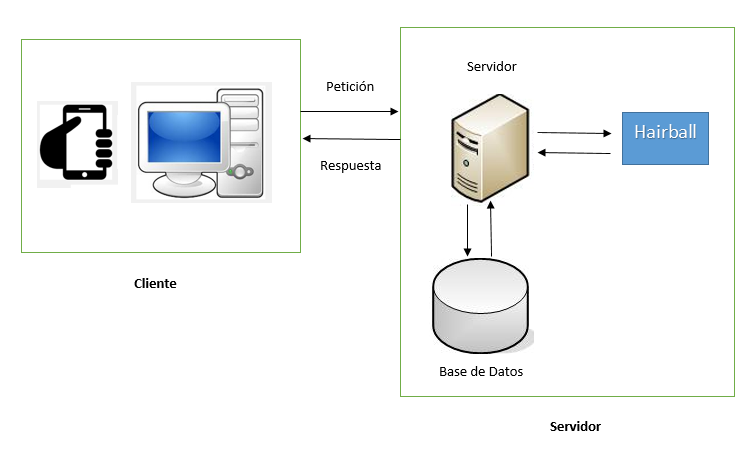
\includegraphics[bb=0 0 800 600, width=18cm, height=9cm, keepaspectratio]{arquitecturascratch.png}
	\caption{Arquitectura de la plataforma Dr. Scratch}
  \label{figura:foro_hilos}
\end{figure}

Se describe cada componente de Dr. Scratch.

\begin{itemize}
  \item Servidor. Se basa principalmente en Django. Django permite la abstracción de la
	base de datos, el modelo vista controlador y la interacción con el componente Front End.
  \item \texttt{Hairball}. Es un framework que permite el análisis de proyectos Scratch. Su uso es
	a través de una consola bash. Hairball se compone de plugins, para usar cada uno se
	tiene que realizar una llamada independiente por consola.
  \item Cliente. Generalmente el acceso a la plataforma se hace mediante un navegador. El
	desarrollo de la parte Front End se realiza conjuntamente con Django y Bootstrap, este
	último permite una funcionalidad responsive lo que permite que el acceso a Dr. Scratch
	puede hacerse por un dispositivo móvil o tablet, sin la pérdida del diseño original. 
\end{itemize}



\section{Diseño e implementación del servidor}
\label{sec:servidor}

El diseño e implementación del servidor se basa en dos partes representativas. Por un lado todo lo
correspondiente a la plataforma web con Django y por otro la incorporación de la funcionalidad de
\texttt{Hairball} y su correspondiente tratamiento de información. \\

Como se mencionó el desarrollo del servidor se realiza mediante Django. Cuando se instala un proyecto
Django se generan varios ficheros entre los que destacan models.py, urls.py, views.py, settings.py.
En el fichero settings.py principalmente se gestiona la configuración con middlewares, base de datos,
paths para directorios estáticos, especificación de la app, en nuestro caso Dr. Scratch app, y 
dependencias con otras aplicaciones. \\

En el fichero models.py es donde se especificará el modelo de datos de la aplicación Django. Gracias 
al potencial del framwork esta definición se realiza como si fuesen clases. La clase se corresponde 
con una tabla y los atributos con campos de estas tablas. \\

Para diseñar las URLs de la aplicación se utiliza el fichero urls.py, donde se especifica cada url y
su correspondiente método en el fichero views.py. Mencionar que la especificación de url admite 
expresiones regulares para capturar más diversidad de recursos.
Por último, en el fichero views.py se crean los métodos que darán la lógica a la aplicación, y esta
estrechamente relacionado con los ficheros urls.py y models.py.


\subsection{Conexión con Hairball}
\texttt{Hairball} provee la salida de datos a través de la consola. Para cada plugin de Hairball se 
debe hacer una llamada a través de la consola. En esta sección se detalla con ejemplos las salidas 
de cada uno de los plugins usados en Dr.Scratch, ya que esto contribuirá al entendimiento del modelo 
de datos del proyecto. \\ \\ 

Cada uno de los plugins se ejecutan a través de una consola bash y su modo de uso es el siguiente.

\begin{center}
hairball -p "`plugin-hairball"' "`nombre-proyecto-formato-sb2"'
\end{center}

Cabe recordar que los proyectos analizados deben ser obligatoriamente de extensión sb2, que se 
corresponde con el tipo de extensión de la última actualización Scratch, 2.0. Para proyectos de 
versiones inferiores de Scratch, existe la posibilidad de transformarlos en formato sb2 y poder
usar Dr. Scratch para el análisis. Esto se explicará en el capítulo 5, ya que, es un nuevo
desarrollo hecho por el equipo Dr. Scratch. \\

Para evaluar las salidas de \texttt{Hairball} se usará el proyecto Scratch test-project.sb2, 
un desarrollo descargado aleatoriamente a través de la nube de 
Scratch.\footnote{\url{scratch.mit.edu/}} \\

Para usar el plugin DeadCode se hace la siguiente llamada.
\begingroup
\fontsize{8pt}{9pt}\selectfont
\begin{verbatim}
hairball -p blocks.DeadCode test-project.sb2 
test-project.sb2 
'Stage': [kurt.Script([ 
    kurt.Block('whenIReceive', u'never'), 
    kurt.Block('startScene', u'castle')], pos=(366, 155)), 
           kurt.Script([  
    kurt.Block('whenIReceive', u'yeppers'), 
    kurt.Block('startScene', u'castle')], pos=(229, 243)), 
           kurt.Script([ 
    kurt.Block('whenIReceive', u'no'), 
    kurt.Block('startScene', u'castle')], pos=(85, 312))] 
\end{verbatim}
\endgroup

De la salida se deduce que para el proyecto Scratch test-project.sb2 existen 6 bloques de código
muerto, es decir, 6 bloques que no llegan a ejecutarse, y estos bloques pertenecen a 3 scripts. 
En el estado del arte se describió que \texttt{Hairball} estaba desarrollado sobre Kurt, en la
salida de este plugin se puede apreciar de que manera trabaja Kurt y sus ventajas. Otro valor
que se almacenará en base de datos en versiones futuras de la plataforma será la información de 
la posición asociada a los bloques que no se ejecutan en el flujo del programa. \\ 

Para el uso del plugin AttributeInitialization se presenta la siguiente salida:

\begingroup
\fontsize{8pt}{8pt}\selectfont
\begin{verbatim}
hairball -p initialization.AttributeInitialization test-project.sb2 
test-project.sb2
{u'frozen_elsa_by_meddek-d6w674h': {'position': 2, 'size': 0, 'costume': 0, 'visibility': 2, 'orientation': 0}, 
u'Sprite8': {'position': 0, 'size': 0, 'costume': 0, 'visibility': 2, 'orientation': 0}, 
u'ElsaPose': {'position': 2, 'size': 0, 'costume': 0, 'visibility': 2, 'orientation': 0}, 
u'Sprite4': {'position': 2, 'size': 0, 'costume': 0, 'visibility': 2, 'orientation': 0}, 
'stage': {'background': 2}, 
u'Sprite2': {'position': 0, 'size': 0, 'costume': 0, 'visibility': 2, 'orientation': 0},
 u'Sprite3': {'position': 2, 'size': 0, 'costume': 1, 'visibility': 2, 'orientation': 0},
 u'Sprite1': {'position': 2, 'size': 0, 'costume': 0, 'visibility': 2, 'orientation': 0}}
\end{verbatim}
\endgroup

Este plugin busca propiedades de los personajes que son modificadas en algún punto del 
proyecto, pero que no se inicializaron al comenzar el flujo del programa. Las propiedades 
de los personajes en general son: position, size, costume, visibility, orientation. 
Por cada propiedad analizada de cada personaje se muestra un valor parametrizado: un valor 
0 si no ha modificado la propiedad, un 1 si se modifica pero no se inicializa, 2 si se inicializa
correctamente. Por lo tanto como se observa en la salida del plugin las propiedades que tienen
 un valor de 1 caen un error de programación, y serán las propiedades que se almacenarán en la
base de datos para su posterior extracción. Mencionar que para el objeto stage, la única 
propiedad de la que dispone es background. Esta es la única excepción que no cumpla con 
las propiedades de los personajes antes mencionada. \\


Para usar el plugin SpriteNaming se hace la siguiente llamada.
\begingroup
\fontsize{8pt}{9pt}\selectfont
\begin{verbatim}
hairball -p convention.SpriteNaming test-project.sb2 
test-project.sb2
5 default sprite names found:
Sprite2
Sprite8
Sprite1
Sprite4
Sprite3
\end{verbatim}
\endgroup

Este plugin busca los personajes del proyecto que han mantenido el nombre por defecto. En
la salida se puede observar un listado de los nombres de esto personajes. Lo que se 
almacenará dentro de la base de datos será el nombre por defecto que aparece en el listado
de la salida del plugin. En el ejemplo anterior: Sprite2, Sprite8, Sprite1, Sprite4, Sprite3. \\  

Para usar el plugin DuplicateScripts se hace la siguiente llamada.
\begingroup
\fontsize{8pt}{9pt}\selectfont
\begin{verbatim}
hairball -p duplicate.DuplicateScripts test-project.sb2 
test-project.sb2
test-project.sb2
1 duplicate scripts found
['when @greenFlag clicked', 'forever', 'if s then s else s',
'hide', 's = s', 'backdrop name']
0 own defined blocks
\end{verbatim}
\endgroup

Este plugin busca programas repetidos en el proyecto, que deben ser implementados por un
método definido por el creador del proyecto. Lo que se almacenará será una variable entera
con el número de programas repetidos. \\

Este plugin busca los personajes del proyecto que han mantenido el nombre por defecto. En
la salida se puede observar un listado de los nombres de esto personajes. Lo que se 
almacenará dentro de la base de datos será el nombre por defecto que aparece en el listado
de la salida del plugin. En el ejemplo anterior: Sprite2, Sprite8, Sprite1, Sprite4, Sprite3. \\


Por último, se detalla el plugin que ofrece resultados cuantificables del pensamiento 
computacional, y es el más importante desde el punto de vista de información relevante
al usuario, el plugin Mastery.

\begingroup
\fontsize{7pt}{8pt}\selectfont
\begin{verbatim}
\texttt{Hairball} -p mastery.Mastery test-project.sb2 
test-project.sb2
{'Abstraction': 2, 'Parallelization': 3, 'Logic': 3, 'Synchronization': 2, 'FlowControl': 2,
'UserInteractivity': 2, 'DataRepresentation': 1}
Total mastery points: 15/21
Average mastery points: 2.14/3
Overall programming competence: Proficiency
\end{verbatim}
\endgroup

Este plugin no tiene presente los errores encontrados en los otros plugins mencionados.
Analiza el proyecto Scratch y asigna una puntuación que cuantifica el grado de expertise
mostrado en la programación para diferentes aspectos del pensamiento computacional: la
abtracción, paralelización, razonamiento lógico, sincronización, control de flujo,
interactividad con el usuario y representación de la información. Cada aspecto tiene
una puntuación máxima de 3, siendo 1 el nivel más básico y 3 un nivel más experto. En
total la suma de los 7 aspectos es 21. El plugin suma los valores obtenidos en cada 
aspecto del pensamiento computacional y en función del resultado sacado asigna un
nivel de maestría para el proyecto analizado, siendo los niveles: básico, en desarrollo
y profesional. Si el proyecto supera está entre 0 y 7 recibeel nivel básico, si está 
entre 7 y 15 está dentro de desarrollo y si es mayor 15 se encuentra en el nivel
profesional. \\

Esto permite una visión de cómo \texttt{Hairball} funciona. Ahora, se debe adaptar estas
salida para hacerlo compatible con tecnologías web, en este punto entra Django.  \\

Django adopta el paradigma modelo vista controlador, y esto permite un desarrollo de 
aplicaciones de forma muy rápida. La funcionalidad de Dr. Scratch radica en varios 
ficheros que genera Django automáticamente cuando se crea un proyecto, estos son el
fichero urls.py, models.py, forms.py y views.py. \\

Para obtener todos las salidas de los plugins se crean métodos dentro del fichero views.py.
Estos métodos se agrupan dentro de un conjunto denominado \emph{procs}. Estos \emph{procs}
cubren la función de parsing de la salida por consola y los nombres de estos métodos se
corresponden y tienen correlación con los plugins de Hairball. Así pues, para conseguir 
los datos del plugin Mastery se construye el \emph{proc} denominado \emph{procMastery}. 
Para todos los \emph{procs} se tiene sólo un parámetro de entrada denominado lines, que se
corresponde con un tipo de dato String que viene representar la salida del terminal. \\

Un visión el \emph{procMastery} se presenta a continuación:
\begingroup
\fontsize{8pt}{9pt}\selectfont
\begin{verbatim}
def procMastery(request,lines):
    """Mastery"""
    dic = {}
    lLines = lines.split('\n')
    d = {}
    d = ast.literal_eval(lLines[1])
    lLines = lLines[2].split(':')[1]
    points = int(lLines.split('/')[0])
    maxi = int(lLines.split('/')[1])
    
    d_translated = translate(request,d)

    dic["mastery"] = d_translated
    dic["mastery"]["points"] = points
    dic["mastery"]["maxi"] = maxi
    return dic
\end{verbatim}
\endgroup

El \emph{proc} asociado al plugin DuplicateScript cuenta el número de programas
repetidos.
\begingroup
\fontsize{8pt}{9pt}\selectfont
\begin{verbatim}
def procDuplicateScript(lines):
    """Return number of duplicate scripts"""
    dic = {}
    number = 0
    lLines = lines.split('\n')
    if len(lLines) > 2:
        number = lLines[1][0]
    dic["duplicateScript"] = dic
    dic["duplicateScript"]["number"] = number
    return dic
\end{verbatim}
\endgroup

El \emph{proc} que se corresponde con el plugin DeadCode busca los bloques que no se
llegan a ejecutar asociados a un script.
\begingroup
\fontsize{8pt}{9pt}\selectfont
\begin{verbatim}
def procDeadCode(lines):
    """Number of dead code with characters and blocks"""
    lLines = lines.split('\n')
    lLines = lLines[1:]
    lcharacter = []
    literator = []
    iterator = 0
    for frame in lLines:
        if '[kurt.Script' in frame:
            # Found an object
            name = frame.split("'")[1]         
            lcharacter.append(name)
            if iterator != 0:
                literator.append(iterator)
                iterator = 0
        if 'kurt.Block' in frame:
            iterator += 1
    literator.append(iterator)

    number = len(lcharacter)
    dic = {}
    dic["deadCode"] = dic  
    dic["deadCode"]["number"] = number
    for i in range(number):
        dic["deadCode"][lcharacter[i]] = literator[i]
  
    return dic
\end{verbatim}
\endgroup

El \emph{proc} que se corresponde con el plugin SpriteNaming es procSpriteNaming. 
Este método almacena los nombres de los personajes a los que el usuario no 
cambio el valor por defecto,
\begingroup
\fontsize{8pt}{9pt}\selectfont
\begin{verbatim}
def procSpriteNaming(lines):
    """Return the number of default spring"""
    dic = {}
    lLines = lines.split('\n')
    number = lLines[1].split(' ')[0]
    lObjects = lLines[2:]
    lfinal = lObjects[:-1]
    dic['spriteNaming'] = dic
    dic['spriteNaming']['number'] = str(number)
    dic['spriteNaming']['sprite'] = lfinal
    return dic
\end{verbatim}
\endgroup

El \emph{proc} que se corresponde con el plugin AttributeInitialization es 
procInitialization. Es el método más complejo, ya que tiene procesar y 
buscar las propiedades de cada personaje, y compararlo con el valor que 
se parametriza como un error.

\begingroup
\fontsize{8pt}{9pt}\selectfont
\begin{verbatim}

def procInitialization(lines):
    """Initialization"""
    dic = {}
    lLines = lines.split('.sb2')
    d = ast.literal_eval(lLines[1])
    keys = d.keys()
    values = d.values()
    items = d.items()
    number = 0
    
    for keys, values in items:
        list = []
        attribute = ""
        internalkeys = values.keys()
        internalvalues = values.values()
        internalitems = values.items()
        flag = False
        counterFlag = False
        i = 0
        for internalkeys, internalvalues in internalitems:
            if internalvalues == 1:
                counterFlag = True
                for value in list:
                    if internalvalues == value:
                        flag = True
                if not flag:
                    list.append(internalkeys)
                    if len(list) < 2:
                        attribute = str(internalkeys)
                    else:
                        attribute = attribute + ", " + str(internalkeys)
        if counterFlag:
            number = number + 1
        d[keys] = attribute      
    dic["initialization"] = d
    dic["initialization"]["number"] = number

    return dic
\end{verbatim}
\endgroup



De este modo, Dr. Scratch transforma las salidas de los plugins a través de \emph{procs}. 
Pero, para poder acceder al sistema operativo desde Django se usa en el proyecto la
librería \emph{os} de Python. La librería \emph{os} permite hacer llamadas de sistema y
ejecutar comandos de bash desde programas Python, y en nuestro caso permite ejecutar las
llamadas a los plugins de Hairball desde el fichero views.py de Django. \\

Dentro del paquete \emph{os} se utiliza la función \emph{read} de la clase \emph{popen}.
A esta función se le pasa una variable tipo String con la correspondiente llamada al 
plugin de Hairball. Volviendo al ejemplo con el plugin Mastery se utiliza la función 
tal que: \\

\begingroup
\fontsize{8pt}{9pt}\selectfont
\begin{verbatim}
os.popen(metricMastery).read()
\end{verbatim}
\endgroup

Siendo metricMastery una variable String con el valor y filename el nombre del fichero
sb2 que representa el proyecto analizado. \\

\begingroup
\fontsize{8pt}{9pt}\selectfont
\begin{verbatim}
metricMastery = "hairball -p mastery.Mastery " + filename
\end{verbatim}
\endgroup

La salida del \emph{proc} es un diccionario construido con los datos relevantes del 
plugin. Posteriormente, se detallará el modelo de datos con el que se observará el
objetivo de cada \emph{proc}. \\

Con la descripción previa se puede hacer una analogía con los distintos \emph{procs}, desde
el punto de vista de la metodologia de uso. Así pues, para el proyecto se construyen, 
además de \emph{procMastery}, los \emph{procs}, \emph{procDuplicateScript}, 
\emph{procSpriteNaming}, \emph{procDeadCode}, \emph{procInitialization} que son usados
para cubrir la captura de datos de los otros plugins. \\

En este punto, se ha explicado como los \emph{procs} funcionan para capturar los datos
de los plugins, pero será otro método el que llame a estos \emph{procs}. Este método 
será \emph{analyzeProject}.

\begingroup
\fontsize{7pt}{8pt}\selectfont
\begin{verbatim}

def analyzeProject(request,file_name):
    dictionary = {}
    if os.path.exists(file_name):
        list_file = file_name.split('(')
        if len(list_file) > 1:
            file_name = list_file[0] + '\(' + list_file[1]
            list_file = file_name.split(')')
            file_name = list_file[0] + '\)' + list_file[1]
        #Request to hairball
        metricMastery = "hairball -p mastery.Mastery " + file_name
        metricDuplicateScript = "hairball -p \
                                duplicate.DuplicateScripts " + file_name
        metricSpriteNaming = "hairball -p convention.SpriteNaming " + file_name
        metricDeadCode = "hairball -p blocks.DeadCode " + file_name 
        metricInitialization = "hairball -p \
                           initialization.AttributeInitialization " + file_name

        #Response from hairball
        resultMastery = os.popen(metricMastery).read()
        resultDuplicateScript = os.popen(metricDuplicateScript).read()
        resultSpriteNaming = os.popen(metricSpriteNaming).read()
        resultDeadCode = os.popen(metricDeadCode).read()
        resultInitialization = os.popen(metricInitialization).read()
        
				#Create a dictionary with necessary information
        dictionary.update(procMastery(request,resultMastery))
        dictionary.update(procDuplicateScript(resultDuplicateScript))
        dictionary.update(procSpriteNaming(resultSpriteNaming))
        dictionary.update(procDeadCode(resultDeadCode))
        dictionary.update(procInitialization(resultInitialization))
        
				#Return a dictionary
				return dictionary
    else:
        return HttpResponseRedirect('/')

\end{verbatim}
\endgroup

En este método se crea una variable diccionario, denominado dictionary, que almacena
toda la información recogida por los diccionarios generados por \emph{procs}. 


\subsection{Modelo de datos}

El modelo de datos tiene como objetivo adecuarse a las salidas de consola de 
\texttt{Hairball}. En el apartado anterior se explicó con detalle como se gestionan 
las salidas de los plugins y como mediante los \emph{procs}, parsers, estos son tratados.
Cabe recordar, que las salidas de estos \emph{procs} son diccionarios. En este capítulo
se detalla el procedimiento de almacenamiento, además de la configuración del sistema de 
base de datos en este proyecto SQlite. \\ 

Una de las principales ventajas de Django es que la conexión con los sistemas de bases
de datos es transparente para el usuario. Simplemente se debe realizar la respectiva 
configuración en el fichero settings.py de la base de datos. Para este proyecto se uso
en primera instancia SQlite, y después se migró a Azure, trabajo realizado por otros 
participantes dentro la iniciativa Dr. Scratch. En este proyecto se limitará la 
descripción con SQLite. \\  
 
Para el entendimiento de los datos dentro de Dr. Scratch se presenta un modelo que 
explica las conexiones de cada una de las estructuras. Como se puede observar en la 
Figura 4.2, la principal tabla en el modelo de datos es Project. La tabla Project 
almacena el nombre del proyecto, la puntuación obtenido según se la descripción 
anterior, el nivel obtenido tras el análisis, la fecha en que se analizó, la versión 
del proyecto analizado con vistas a hacer un seguimiento de la progresión del 
usuario de Dr. Scratch. \\ \\

 \begin{figure}[h]
		\graphicspath{{img/}}
    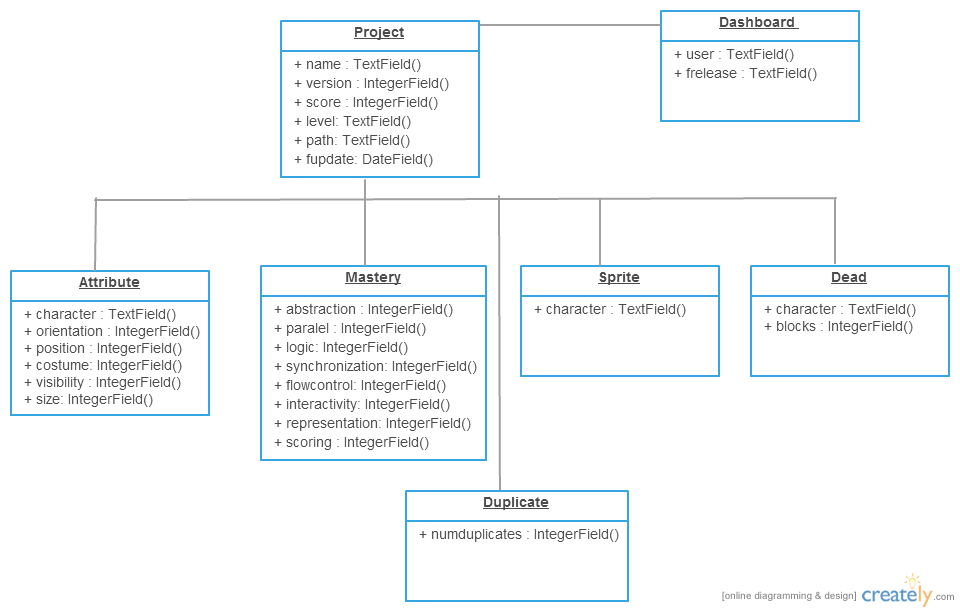
\includegraphics[bb=0 0 800 600, width=14cm, keepaspectratio]{modelo.png}
    \caption{Representación del Modelo de Datos de Dr. Scratch}
    \label{figura:foro_hilos}
 \end{figure}



Como se menciona al inicio del capítulo, cada tabla trata de corresponderse con los
plugins de \texttt{Hairball}. Para el plugin Mastery, se tiene la tabla Mastery, en
la se almacena las puntuaciones referentes a las habilidades de pensamiento 
computacional obtenidos, y además la puntuación obtenida para el proyecto. Estos 
valores son de tipo entero. \\ 

La tabla Attribute guarda las propiedades del personaje que presentan un error en su 
inicialización. Así pues, se parametriza las propiedades generales de los personajes,
orientation, costume, visibility, size, position, todas de tipo entero. Como se 
comentó anteriormente un 1 en las propiedades representa un error. \\

La tabla Sprite almacena el nombre del personaje que se ha dejado por defecto. \\

La tabla Dead almacena el número de bloques de código muerto asociados. Estos bloques
siempre están asociados a un personaje, ya que generalmente pertenecen a scripts, así
que también se guarda el nombre del personaje. \\

La tabla Duplicate almacena el número de programas repetidos existentes en el proyecto. \\

Para la definición del modelo de datos en Django, esto se debe especificar en el fichero
models.py. Como se comentó previamente, la especificación de una tabla se corresponde con
una clase en Python, y los columnas sería los atributos de esta clase. A continuación, se
presenta el modelo de datos en el formato para el framework Django.


\begingroup
\fontsize{9pt}{10pt}\selectfont
\begin{verbatim}
class Project(models.Model):
	name = models.TextField()
	version = models.IntegerField()
	score = models.IntegerField()
	level = models.TextField()
	path = models.TextField()
	fupdate = models.TextField()
	dashboard = models.ForeignKey(Dashboard)
	
class Attribute(models.Model):
	myproject = models.ForeignKey(Project)
	character = models.TextField()
	orientation = models.IntegerField()
	position = models.IntegerField()
	costume = models.IntegerField()
	visibility = models.IntegerField()
	size = models.IntegerField()

class Dead(models.Model):
	myproject = models.ForeignKey(Project)
	character = models.TextField()
	blocks = models.IntegerField()

class Duplicate(models.Model):
	myproject = models.ForeignKey(Project)
	numduplicates = models.IntegerField()

class Sprite(models.Model):
	myproject = models.ForeignKey(Project)
	character = models.TextField()

class Mastery(models.Model):
	myproject = models.ForeignKey(Project)
	abstraction = models.IntegerField()
	paralel = models.IntegerField()
	logic = models.IntegerField()
	synchronization = models.IntegerField()
	flowcontrol = models.IntegerField()
	interactivity = models.IntegerField()
	representation = models.IntegerField()
	scoring = models.IntegerField()	

\end{verbatim}
\endgroup


\section{Diseño e implementación del cliente}
\label{sec:servidor}

Como se menciona al inicio del capítulo para el desarrollo de la parte del cliente se usa
Bootstrap. Se utilizan varios componentes y funcionalidades de este
 framewok\footnote{\url{http://getbootstrap.com/components/}}, como por ejemplo los icons,
buttons, sizing, navs, tabs, thumbnails, alerts. Por ejemplo, para la creación de la 
portada, representada en la Figura 4.3, se utiliza como componente principal un navbar y la
funcionalidad de thumbnails. \\

 \begin{figure}[h]
		\centering
		\graphicspath{{img/}}
    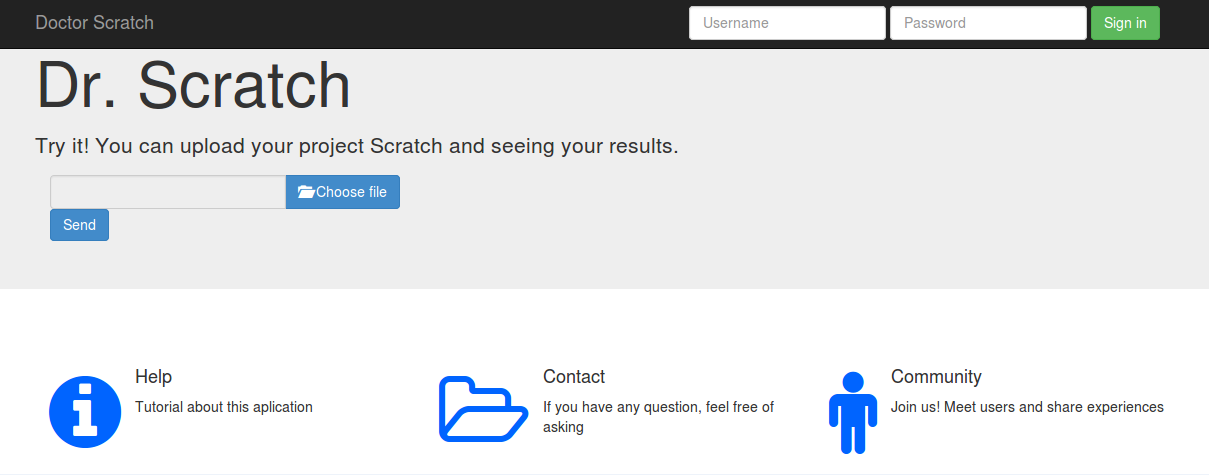
\includegraphics[bb=0 0 800 600, width=15cm, height=8cm, keepaspectratio]{portada.png}
		\caption{Página inicial de Dr. Scratch}
    \label{figura:foro_hilos}
 \end{figure} 

La página principal de Dr. Scratch, Figura 4.3, es una de las primeras 
versiones de portada, pero engloba los componentes de Bootstrap principales 
usadas en las siguientes versiones. Como se puede observar en la imagen existe la 
posibilidad de que un usuario acceda con su cuenta dentro de la plataforma, esta
funcionalidad también es cubierta con Django, que provee herramientas para la 
gestión de usuarios y sesiones dentro del desarrollo de sus aplicaciones. \\ \\ 

En la parte izquierda de la Figura 4.3 se puede apreciar un formulario desarrollado
para que el usuario de la plataforma pueda subir su proyecto Scratch con extensión sb2
a la aplicación para su análisis. Cuando el usuario selecciona el fichero y da clic
a enviar, la petición y el fichero serán entregados al servidor de Dr. Scratch para
su procesado. \\

Si no existió ningun error en la entrega de la petición o problemas con la extensión del
fichero, la siguiente página que es mostrada por la aplicación es la que aparece en la
Figura 4.4. Lo primera que se puede apreciar en esta imagen es la puntuación obtenida 
después del análisis dentro de Dr. Scratch. Además, junto a la puntuación se representa
el nivel de expertise conseguido tras el análisis dentro de la plataforma. Esta 
información es el resultado del proceso que sigue Dr. Scratch, pasando el proyecto por
Hairball, procesando las salidas de consola, almacenando la información y renderizando los
datos de ciertas tablas del modelo de datos, concretamente en este página la de la tabla
Mastery, encargada de gestionar información general de cada proyecto analizado. 


 \begin{figure}[h]
    \centering
		\graphicspath{{img/}}
    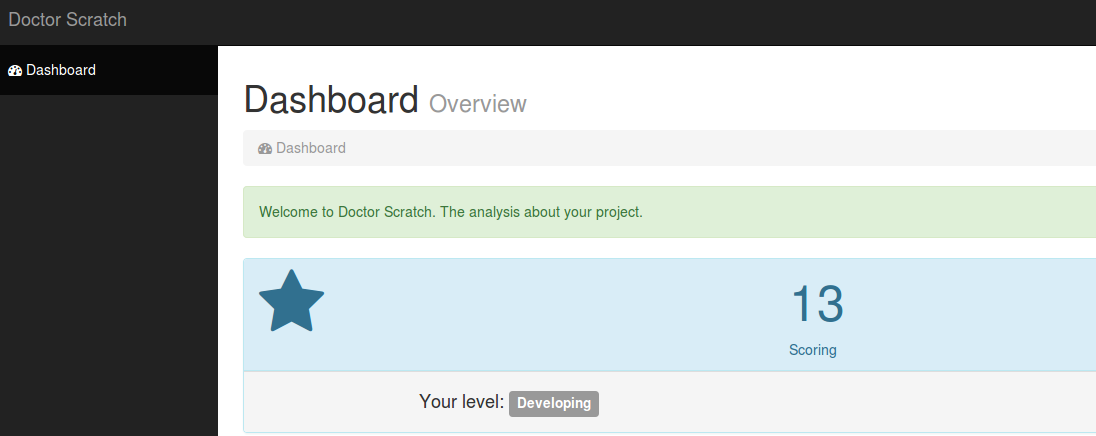
\includegraphics[bb=0 0 800 600, width=16cm, height=8cm, keepaspectratio]{puntuacion.png}
		\caption{Puntuación de proyecto obtenido en Dr. Scratch}
    \label{figura:foro_hilos}
 \end{figure} 


Además, en esta página se representa la información del plugin Mastery. Se detalla
en una tabla los valores obtenidos en cada una de las habilidades pensamiento
computacional: Sincronización, flujo de control, paralelización, abstracción,
interacción con el usuario y lógica. Como se puede apreciar en la figura 4.5, las
puntuaciones no exceden el límite de 3 y la suma de todos las propiedades no excede
el máximo de 21 puntos. Estos criterios se puntuación y asignación de nivel se han
mantenido a lo largo del ciclo de vida de Dr. Scratch. \\

\begin{figure}[h]
  \centering
	\graphicspath{{img/}}
  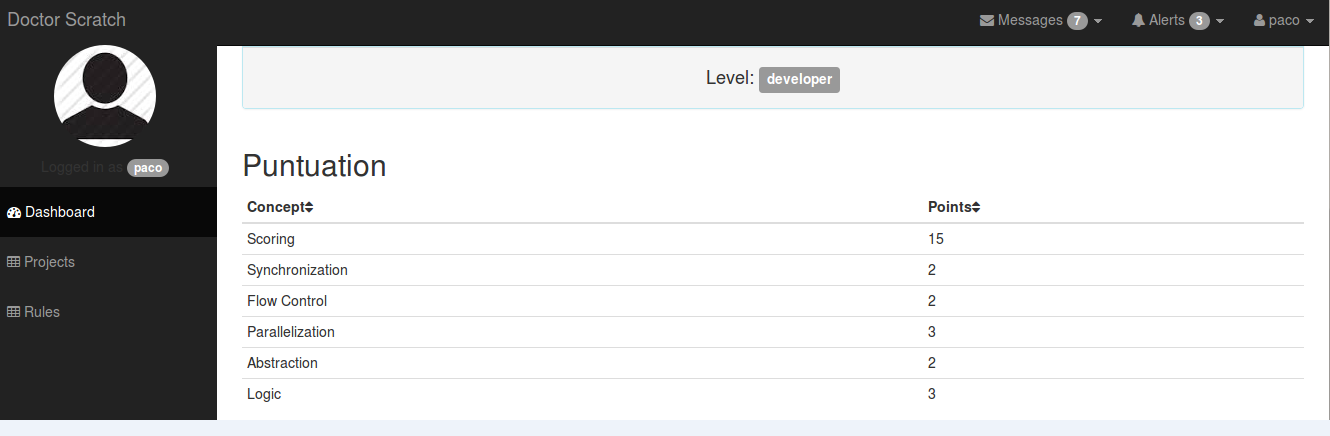
\includegraphics[bb=0 0 800 600, width=18cm, height=8cm, keepaspectratio]{scoring.png}
	\caption{Puntuaciones en habilidades pensamiento computacional para un proyecto}
  \label{figura:foro_hilos}
\end{figure}


Si se sigue el análisis de los resultados renderizados en esta misma página, además de 
lo referenciado anteriormente, se muestra los datos almacenados por las distintas tablas
la base de datos.  Los datos referidos a los plugins, \emph{DuplicateScripts}, 
\emph{SpriteNaming}, \emph{DeadCode} y \emph{AttributeInitialization}. Figura 4.5. \\

Para el plugin \emph{DuplicateScripts} se muestra el número de programas repetidos, sin 
ninguna información agregada. Para \emph{SpriteNaming} se lista los personajes que usan
su nombre por defecto y se muestra la suma de estos personajes. 
Para el plugin \emph{DeadCode} se muestra el nombre del personaje y dentro de éste el 
número de bloques que no se llegan a ejecutar
Para \emph{AttributeInitialization} se muestra el personaje y dentro de este las 
propiedades que no cumplen con su correcta inicialización.

 \begin{figure}[h]
	  \centering
		\graphicspath{{img/}}
    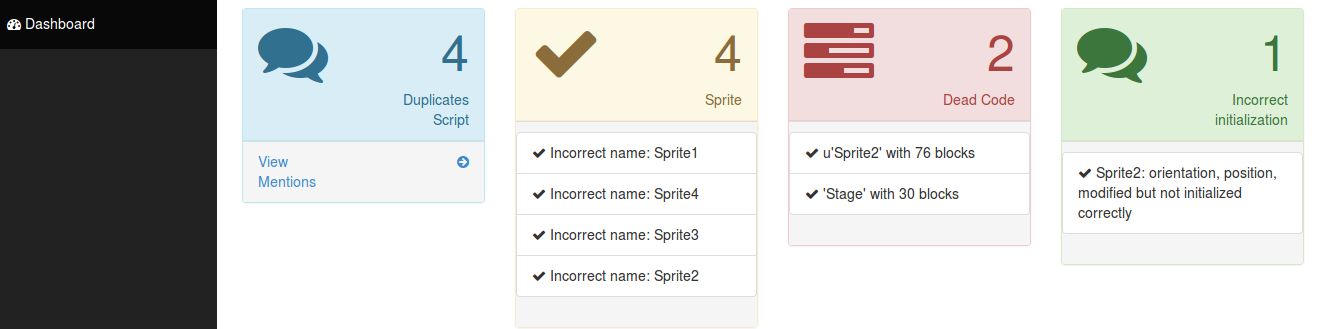
\includegraphics[bb=0 0 800 600, width=18cm, height=7cm, keepaspectratio]{plugins.png}
		\caption{Datos de plugins de Hairball en Dr. Scratch}
    \label{figura:foro_hilos}
 \end{figure} 


El componente principal de Bootstrap usado en esta página es \emph{Thumbnails}. Este
componente permite crear de manera sencilla display grids, \emph{cajas}, y dentro de
estas se puedan colocar imágenes, vídeos y texto. En nuestro caso lo usamos para
colocar los datos referentes a los plugins que se han mencionado anteriormente.  \\

Esta información mostrada en las imágenes adjuntas es para un usuario no registrado.
Para un usuario registrado es posible otorgarle más funcionalidades. Dentro de las
primeras versiones de Dr. Scratch el usuario registrado tiene un dashboard o cuadro
de mandos donde puede tener una visión rápida de todos los proyectos analizados y de
sus respectivos niveles y puntuaciones. \\

Este cuadro de mandos se puede observar en detalle en la Figura 4.7. Consta de tres 
contenedores principales: panel superior, panel izquierdo y panel central.
En el panel izquierdo, el usuario registrado tiene disponible tres enlaces: Dashboard,
Projects y Rules. Dashboard es el enlace que te permite acceder a los portles generales
para la categorización de los proyectos. Projects es un enlace que te lleva a una 
página donde se muestra cada uno de los proyectos del usuario, mostrando la puntuación
obtenida. Por último, el enlace Rules te lleva a una página donde se describe los niveles
dentro de Dr. Scratch, y como se puede alcanzar cada uno de ellos. \\ \\ \\

La página Dashboard se corresponde con la Figura 4.7. En este punto, el usuario de 
Dr. Scratch tiene la posibilidad de tener una visión más general de todos sus proyectos
analizados almacenados dentro de la plataforma. Este cuadro de mandos está formado por
tres bloques principales. El primer bloque es un gráfico estadístico que obtiene de 
base de datos todos los proyectos y los categoriza por el nivel obtenido tras el 
análisis con la herramienta, es decir, básico, desarrollo o profesional. \\ 

\begin{figure}[h]
  \centering
	\graphicspath{{img/}}
  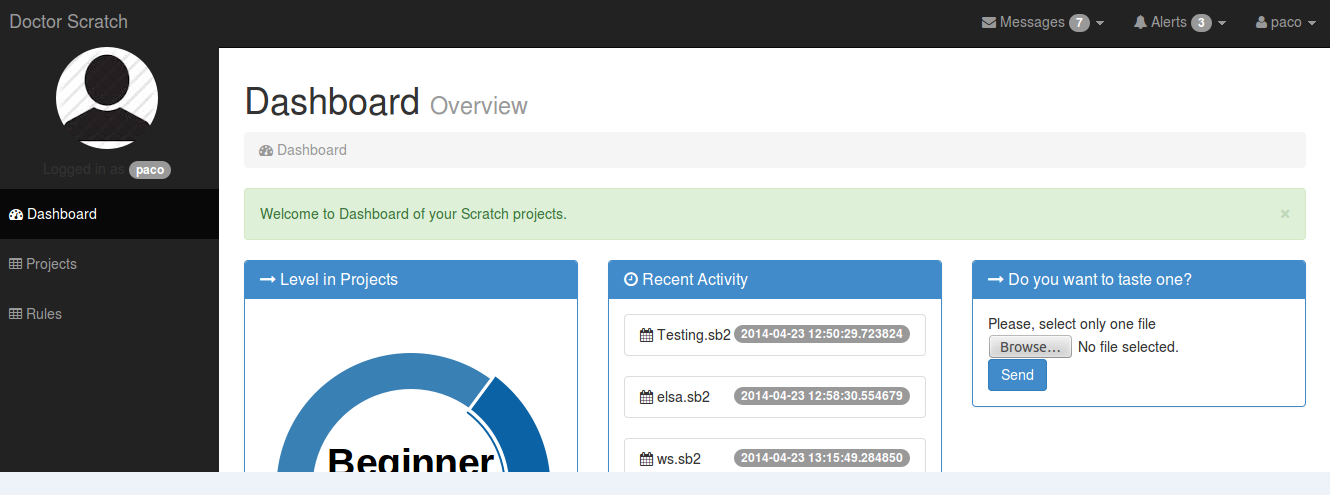
\includegraphics[bb=0 0 800 600, width=18cm, height=9cm, keepaspectratio]{dashboardprincipal.png}
	\caption{Cuadro de mandos para usuario registrado en Dr. Scratch}
  \label{figura:foro_hilos}
\end{figure}


El siguiente bloque es el encargado de mostrar toda la actividad del usuario dentro de Dr. Scratch.
Ordena esta actividad cronológicamente y estas actividades pueden ser subir proyectos 
nuevos a la plataforma, actualizar un proyecto ya existente o realizar un comentario sobre
otros usuarios registrados dentro la plataforma. \\

El último bloque que se puede apreciar es donde el usuario tiene habilitado un formulario 
para subir el proyecto Scratch que quiere ser analizado. Este bloque es casi idéntico al 
que tiene un usuario no registrado que  pretende usar la herramienta para analizar sus
 proyectos Scratch. \\ 

En el panel superior se tiene habilitado los enlaces para que el usuario pueda modificar
propiedades de su cuenta, visualizar sus mensajes, ver alertas. Esto se corresponde con
la primera versión de plantilla Bootstrap, y la lógica está pendiente como futuras tareas
de desarrollo. \\ 



Como se describió previamente, en la panel izquierdo de la página del usuario registrado 
existen tres enlaces. El enlace Dashboard ha sido descrito haste el momento. Si el usuario
selecciona el enlace Projects podrá acceder a la Figura 4.8.  

\begin{figure} [h]
  \centering
	\graphicspath{{img/}}
  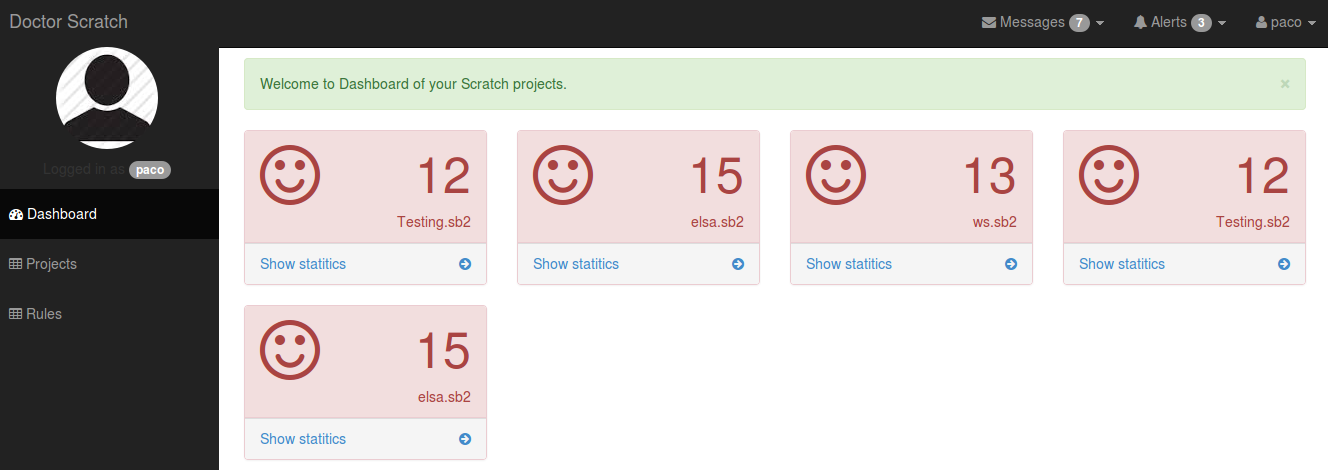
\includegraphics[bb=0 0 800 600, width=18cm, height=8cm, keepaspectratio]{proyectos.png}
	\caption{Listado de proyectos de un usuario registrado en Dr. Scratch}
  \label{figura:foro_hilos}
\end{figure}


En esta página los paneles izquierdo y superior se mantienen iguales, y el que cambiará será
el panel central. En este panel se podrá consultar todos los proyectos analizados por el usuario. 
Los proyectos son mostrados con su nombre completo y la puntuación obtenido tras el análisis. 
En cada ítem de proyecto se habilita un enlace que redirige a una página que muestra en detalle
toda la información extraída de los plugins. Esta página será idéntica a la que se muestra a un
usuario no registrado. En futuros desarrollos se tiene como objetivo que la página que muestra
las salidas de \texttt{Hairball} también pueda sugerir como mejorar su progresión dentro de la
plataforma. Este desarrollo también será llevado a cabo por el equipo Dr. Scratch en versiones
superiores de la aplicación.  \\ \\ 


El último enlace del panel izquierdo es \emph{Rules}. Rules es una página que muestra
las reglas estipuladas para la adjudicación del nivel en Dr. Scratch. Como se menciona
anteriormente, existen tres niveles dentro de Dr. Scratch: básico, en desarrollo y 
profesional. En un principio, los límites para saltar de nivel eran 10 para pasar de 
básico a desarrollo y 15 para superar desarrollo y conseguir el nivel profesional. Este
aspecto es uno de los que ha variado en la versión actual de Dr. Scratch, actualmente
un usuario de nivel básico está entre 0-7, mientras que un usuario en desarrollo se
encuentra en el rango 7-15, y para los que superan el 15 el nivel será profesional.

\begin{figure}[h]
  \centering
	\graphicspath{{img/}}
  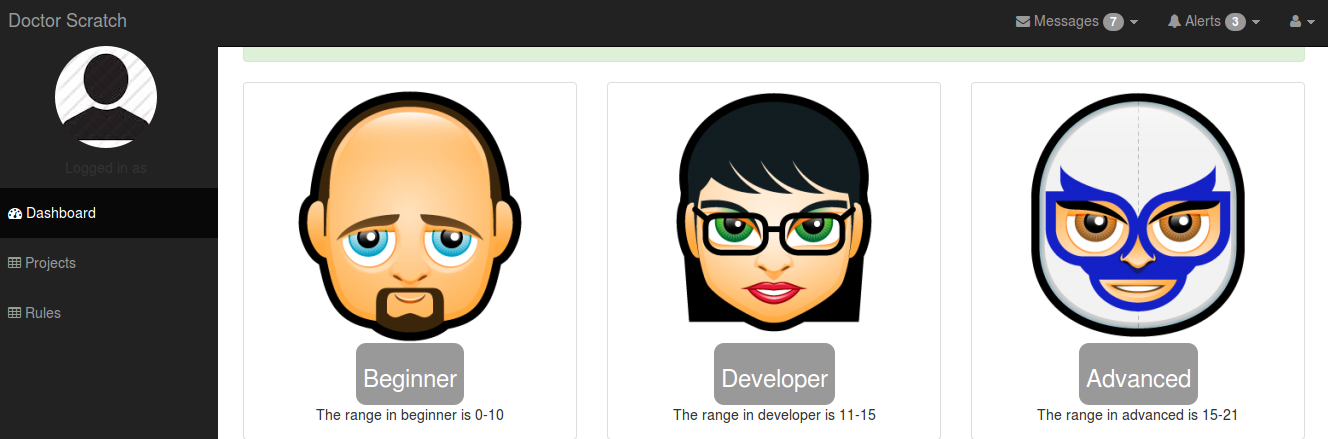
\includegraphics[bb=0 0 800 600, width=18cm, height=8cm, keepaspectratio]{niveles.png}
	\caption{Niveles dentro de Dr. Scratch}
  \label{figura:foro_hilos}
\end{figure}

Uno de los objetivos del proyecto es aplicar un seguimiento de la progresión del 
usuario mientra usa la plataforma. El uso de niveles permite que el usuario se posicione
y asuma el reto de superar niveles, y así conseguir mayor visibilidad dentro de Dr. 
Scratch. Es una tarea pendiente el poder enlazar técnicas de ludificación, el mecanismo
de seguimiento del proceso y la integración del componente de red social. \\ \\


\section{Implementación de plugin firefox para Dr. Scratch}
\label{sec:servidor}

Uno de los detalles más importantes dentro de las aplicaciones web es la facilidad de 
uso para los usuarios. Desde la iniciativa Dr. Scratch se valoró crear plugins para
los navegadores más usados: Chrome y Firefox. \\

Para Chrome existen librerías para el desarrollo de extensiones, equivalente de plugin
en Firefox, se investigó la manera de interactuar con los componentes que ofrecían
las librerías de Chrome y tienen mucha correlación con Firefox. Pero, en el punto
de entrega de este proyecto no se llegó a implementar una solución, pese a la
investigación y pruebas realizadas. \\

En Firefox la facilidad que te otorga el SDK hace que el desarrollo de plugins sea 
sencillo y rápido de hacer. En principio las librerías vienen comprimidas en un
fichero tar.gz. Para descomprimir se puede usar el comando bash tar -xf addon-sdk.tar.gz.
Una vez hecha la descompresión, vamos al directorio y ejecutamos source bin/activate.
Esto crea un nuevo prompt adaptado para el desarrollo de plugins.\\ \\

Para crer una app nueva, o plugin nuevo se sigue la siguiente ejecución de comandos:
\begingroup
\fontsize{8pt}{9pt}\selectfont
\begin{verbatim}
mkdir my-addon
cd my-addon
cfx init
\end{verbatim}
\endgroup

Siendo my-addon el nombre del plugin. En el caso del plugin de Dr. Scratch el nombre
recibido es drscratch-tool. Cuando se ejecuta cfx init se genera un nuevo directorio
con la siguiente estructura de ficheros:
\begingroup
\fontsize{8pt}{9pt}\selectfont
\begin{verbatim}
|--data
|   |--css
|   |--js
|   |--icon32.jpg
|--lib
|   |--main.js
|--test
|   |--test-main.js
|--package.json
\end{verbatim}
\endgroup

En el fichero json se especifica el nombre que tendrá el plugin, así como una 
descripción, versión y tipo de licencia. La estructura del fichero json es: \\

\begingroup
\fontsize{8pt}{9pt}\selectfont
\begin{verbatim}
{
  "name": "drscratch-tool",
  "title": "drscratch-tool",
  "id": "jid1-sALq5AVB1uk6GQ",
  "description": "a basic add-on",
  "author": "",
  "license": "MPL 2.0",
  "version": "0.1"
}
\end{verbatim}
\endgroup

El fichero donde escribimos la lógica de la aplicación será main.js. Para el desarrollo
del plugin se ha utilizado varios paquetes del SDK. Por ejemplo, para crear un panel
se usa el paquete panel, para el control de las pestañas del navegador se usa el 
paquete tabs. Pero, el paquete más importante es request, que proporciona la 
funcionalidad de realizar peticiones mediante AJAX a cualquier servidor, en este caso
el servidor de Dr. Scratch. \\
\begingroup
\fontsize{8pt}{9pt}\selectfont
\begin{verbatim}
// Panel
var data = require("sdk/self").data;
var panel = require("sdk/panel").Panel({
	contentURL: data.url("text-entry.html"),
	width: 500,
	height: 300,
	contentStyleFile: data.url("css/drscratch.css"),
  contentScriptFile: [
        data.url("js/jquery-2.1.3.min.js"),
        data.url("get-text.js"), 
  ]
});

// Get the active tab url
var tabs = require("sdk/tabs");

// Create request to DrScratch
var Request = require("sdk/request").Request;

// Create a button
require("sdk/ui/button/action").ActionButton({
	id: "show-panel",
	label: "Show Panel",
	icon: {
		"16": "./icon-16.png",
		"32": "./icon-32.png"
	},
    onClick: handleClick
});


function handleClick(state){
	var url = tabs.activeTab.url;
	var lurl = url.split("/");
	var idproject = lurl[4];
	var url4scratch = "http://localhost:1234/pluginAnalysis/" + idproject;
	var doctor = Request({
	url: url4scratch,
	onComplete: function (response) {
		var gresponse = response.text;
		panel.port.emit("gresponse", gresponse);
		console.log("estoy en request##");
		}
	});
	doctor.get();
	panel.show();
}

panel.on("show", function() {
panel.port.emit("show");
});
\end{verbatim}
\endgroup

Mencionar que el idProject es recogido mediante la funcionalidad del paquete tabs
que recoge la url de la tab activa. Una vez obtenida se parsea hasta conseguir
el identificador del proyecto Scratch. Esta petición será recogido por el servidor 
Django, y procesada por un método que procesa peticiones AJAX. 

%%%%%%%%%%%%%%%%%%%%%%%%%%%%%%%%%%%%%%%%%%%%%%%%%%%%%%%%%%%%%%%%%%%%%%%%%%%%%%%%
%%%%%%%%%%%%%%%%%%%%%%%%%%%%%%%%%%%%%%%%%%%%%%%%%%%%%%%%%%%%%%%%%%%%%%%%%%%%%%%%
% RESULTADOS %
%%%%%%%%%%%%%%%%%%%%%%%%%%%%%%%%%%%%%%%%%%%%%%%%%%%%%%%%%%%%%%%%%%%%%%%%%%%%%%%%

\cleardoublepage
\chapter{Resultados}

El desarrollo de Dr. Scratch ha tomado una nueva dimensión con la inclusión de nuevos 
desarrolladores para el soporte y programación de nuevas funcionalidades. Estos 
participantes son estudiantes que pertenecen a la universidad Rey Juan Carlos. Gracias
a ellos y a la colaboración de los cofundadores de la comunidad Programamos,
Dr. Scratch pudo dar un salto cualitativo en su presentación, su despliegue dentro 
de la plataforma Azure y sobretodo en la difusión y pruebas de la plataforma en 
distintos eventos a lo largo del año. En este capítulo se detalla el estado actual de 
la plataforma Dr. Scratch, mencionando cada aportación de las nuevas personas que se 
integraron a la iniciativa, así como la dinámica de trabajo que se adoptó para la 
ejecución de las nuevas funcionalidades.

\subsection{Nuevo equipo de trabajo de Dr. Scratch}

La inclusión de nuevas personas al proyecto beneficia considerablemente a la 
consecusión de objetivos y la búsqueda de nuevas ramas de innovación dentro de la
iniciativa. A lo largo del desarrollo del proyecto, el trabajo en equipo implicó
un factor añadido, la organización. Por esta razón se adoptó una metodología de 
gestión para la organización de las tareas que cada integrante del equipo realizaría. 
Con el objetivo de centralizar y automatizar todo esta organización se utilizó
la herramienta \emph{Trello}.  

\emph{Trello} permite seguir un modelo Kanban, en el se organizan espacios, y en
cada espacio se encuentran tareas. Los espacios dentro de Dr. Scratch son Doing, ToDo,
Waiting an event y MidTerm.

\begin{figure}
	\centering
	\graphicspath{{img/}}
  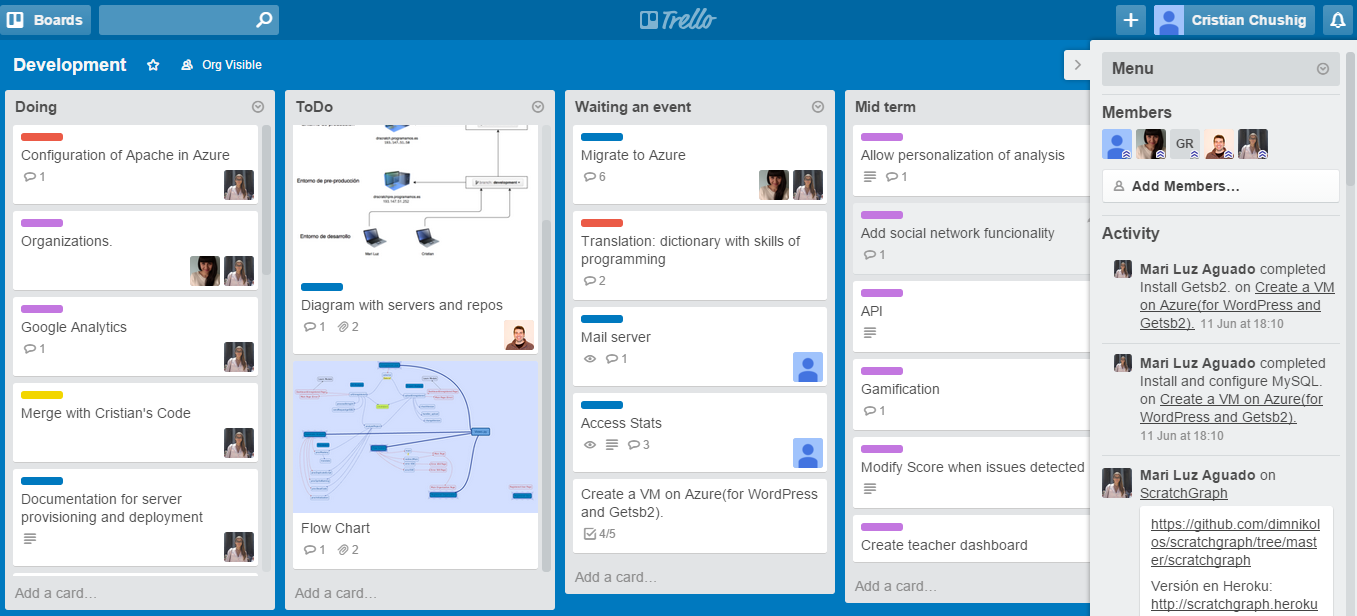
\includegraphics[bb=0 0 800 600, width=18cm, height=9cm, keepaspectratio]{trello.png}
	\caption{Herramienta para gestión de tareas en Dr. Scratch}
  \label{figura:foro_hilos}
\end{figure}


Los participantes dentro de esta herramienta pueden añadir tareas, inscribirse
a tareas y cambiar el estado de estas. Estas tareas son desplazadas en función
del estado en que se encuentre. Si por ejemplo, una tarea acaba de ser creada
estará en el espacio Doing, si un usuario se asigna la tarea y la termina 
satisfactoriamente está tarea será movida a ToDo. \\

Toda la actividad dentro de \emph{Trello} es recogida dentro de un histórico,
que permite tener una visibilidad del trabajo realizado por cada integrante del
equipo. Además, esta forma de trabajar con un métoo gráfico permite identicar
rápidamente tareas que están con retraso, tareas pendientes o tareas que no
se consiguen. \\

Así pues, este es el mecanismo con el que se ha gestionado el trabajo en equipo
de los desarrolladores. Pese a que Dr. Scratch podía ejecutarse correctamente
sobre una máquina local, el siguiente nivel era llevar este correcto funcionamiento 
a servidores en donde usuarios pudiesen valorar la plataforma, además de comprobar 
las limitaciones de la arquitectura y de encontrar posibles \emph{bugs} dentro del código. \\ \\

Uno de los primeros pasos fue instalar todo el ecosistema Dr. Scratch en un servidor de 
la universidad para que usuarios pudiesen probar la plataforma. Este trabajo fue 
ejecutado por dos estudiantes que se unieron a la iniciativa entre el pasado año y el 
actual, y tuvieron que lidiar con los problemas de administración, instalación y 
conexión con una nueva base de datos y sobretodo hicieron la labor de testing de la 
plataforma. Esto fue hito importante, ya que gracias a que Dr. Scratch estaba almacenado
dentro de los servidores de la universidades, ahora se podían hacer pruebas reales
con un grupo de usuarios. \\

Una de las primeras pruebas que se realizón con Dr. Scratch fue en MediaLab Prado con
un número importante de profesores de instituto, que deseaban aprender acerca de 
Scratch, sobre la programación a través de un entorno gráfico, y además Dr. Scratch. \\

En esta prueba se pudo comprobar que las peticiones realizadas sobre Dr. Scratch no 
eran respondidas al cien por ciento, debido a las limitaciones del servidor. Así pues,
se opta por migrar toda el software de Dr. Scratch a la tecnología Azure. \\

Azure permite tener máquinas virtuales en la nube, además de un almacenamiento importante
para datos. En este punto, el trabajo de migración fue realizo por el equipo Scratch y no
se corresponde a hitos logrados en el proyecto.


\subsection{Estado actual de Dr. Scratch}


Una de las contribuciones de la comunidad \emph{Programamos} a la iniciativa fue el 
desarrollo de la plantilla de Bootstrap presente en la última versión disponible en
la red. Como se puede apreciar en la Figura 5.2, la presentación de Dr. Scratch
adquirió un grado de calidad alto, pero sigue la misma estructura que tenía la primera
versión de plantilla Bootstrap. \\

\begin{figure}[h]
	\centering
	\graphicspath{{img/}}
  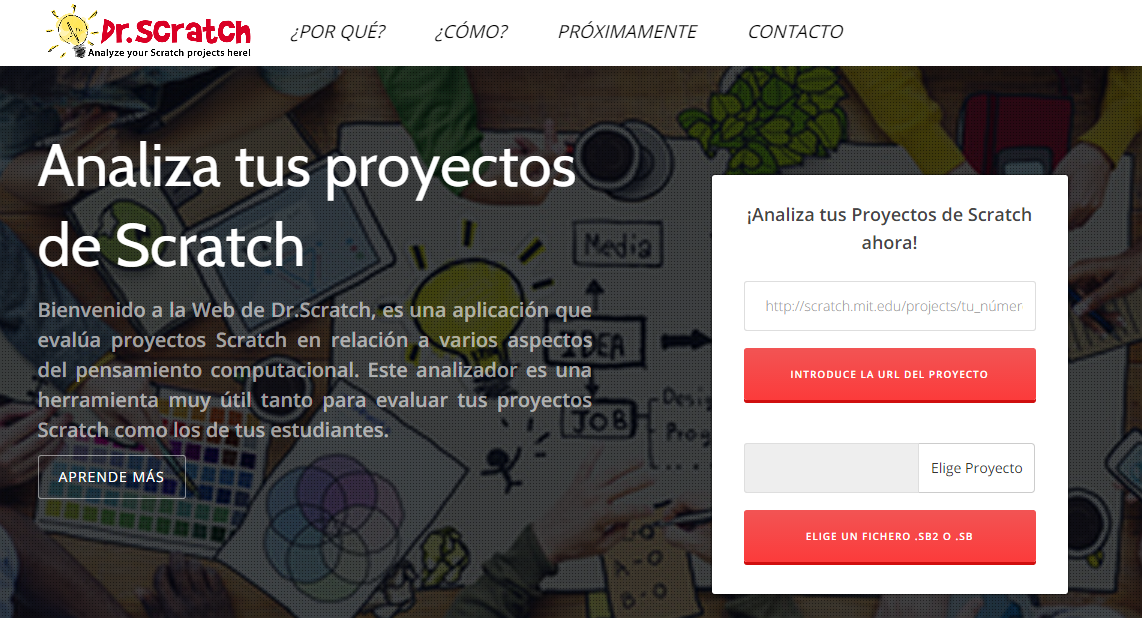
\includegraphics[bb=0 0 800 600, width=18cm, height=8cm, keepaspectratio]{drscratchactual.png}
	\caption{Estado actual de Dr. Scratch}
  \label{figura:foro_hilos}
\end{figure}

La creación de un formulario para poder subir el fichero se mantiene, añadido claro
el \emph{Look and Feel} de la nueva plantilla. Pero aquí se añade un nuevo componente
en el formulario, una entrada de texto, en el que el usuario puede introducir el 
identificador del proyecto para ser analizado. \\

Dr. Scratch hará uso de una herramienta de código abierto que permite descargar todos
los componentes de un proyecto Scratch, simplemente conociendo el identificador del
proyecto asignado por la plataforma de Scratch. Esta herramienta recibe el nombre de
getSb2, y como su nombre indica obtiene un proyecto con formato sb2. \\

Esta herramienta está desarrollada sobre NodeJS, y en un principio se hacía uso del
servicio, ya que estaba disponible siempre en la red. Pero, valorando las limitaciones
de la herramienta en términos de conexiones que es capaz de soportar simultáneamente, 
se optó por hacer una réplica y almacenar una copia dentro de Azure. \\

En el transcurso del proyecto también se decidió hacer una plataforma multilenguaje. 
Para ello, se usó la funcionalidad que proporciona Django para hacer traducciones. 
Esta fase de la iniciativa la desarrolló el equipo de Dr. Scratch. Hubo algunos
inconvenientes, pero se logró mantener una versión en inglés y otra en español, de
acuerdo a la configuración de navegador que se esté usando durante la sesión en la
plataforma. \\  \\ \\


Dentro de las funcionalidades que están en progreso, está las cuentas de los profesores.
Una buena idea para que los profesores puedan usar la herramienta junto a sus alumnos
es proporcionar una interfaz en la que pueda crear classrooms. Los alumnos pueden 
suscribirse a estos grupos para poder participar del reto que envía el profesor.
Los alumnos suben sus proyectos que solucionan el reto lanzado, y el profesor puede 
corregir de manera rápida los proyectos. \\

Además, se tiene en mente que el profesor tenga un cuadro de mandos, en la que pueda
valorar qué alumnos necesitan más ayuda que otros. Esta nueva funcionalidad se mezclaría
con un trabajo futuro del seguimiento del proceso del usuario.


\begin{figure}
	\centering
	\graphicspath{{img/}}
  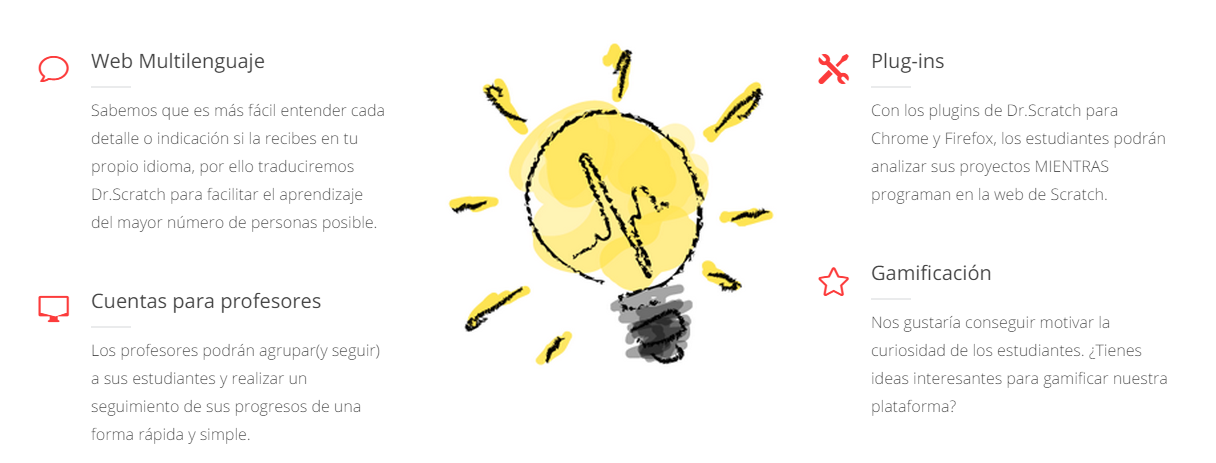
\includegraphics[bb=0 0 800 600, width=18cm, height=8cm, keepaspectratio]{nuevasfuncionalidades.png}
	\caption{Nuevas funcionalidades Dr. Scratch}
  \label{figura:foro_hilos}
\end{figure}

Por último se deja otra captura de la última versión de Dr. Scratch, Figura 5.4. Aquí,
puede verse un vídeo demostrando como usar la plataforma y está orientada a un público 
más general.

\begin{figure}
	\centering
	\graphicspath{{img/}}
  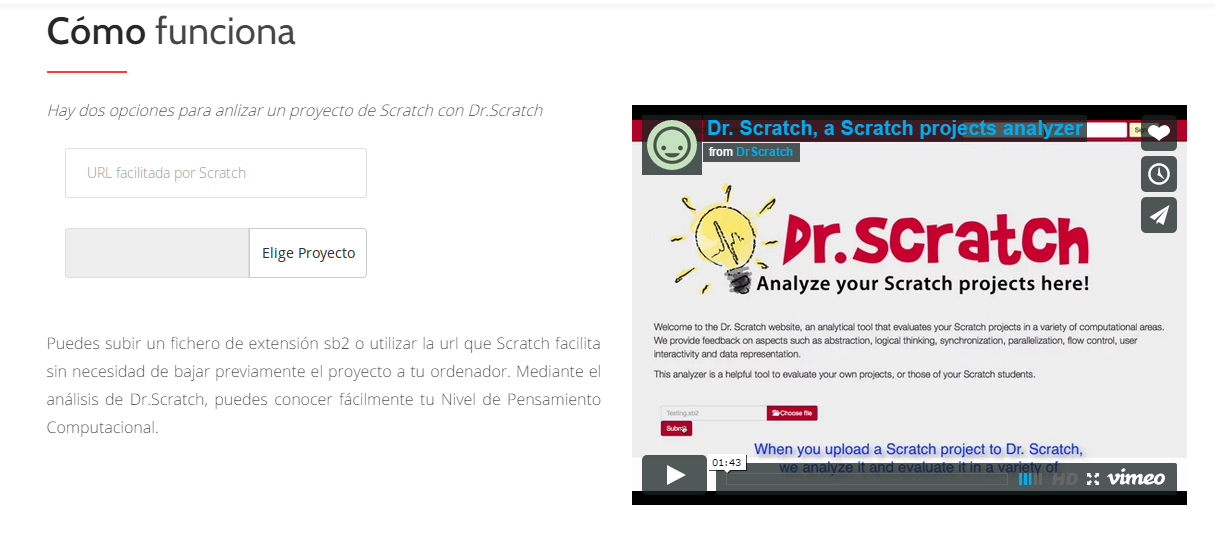
\includegraphics[bb=0 0 800 600, width=18cm, height=8cm, keepaspectratio]{comofunciona.png}
	\caption{Herramienta para gestión de tareas en Dr. Scratch}
  \label{figura:foro_hilos}
\end{figure}




%%%%%%%%%%%%%%%%%%%%%%%%%%%%%%%%%%%%%%%%%%%%%%%%%%%%%%%%%%%%%%%%%%%%%%%%%%%%%%%%
%%%%%%%%%%%%%%%%%%%%%%%%%%%%%%%%%%%%%%%%%%%%%%%%%%%%%%%%%%%%%%%%%%%%%%%%%%%%%%%%
% CONCLUSIONES %
%%%%%%%%%%%%%%%%%%%%%%%%%%%%%%%%%%%%%%%%%%%%%%%%%%%%%%%%%%%%%%%%%%%%%%%%%%%%%%%%

\cleardoublepage
\chapter{Conclusiones}
\label{chap:conclusiones}


\section{Consecución de objetivos}
\label{sec:consecucion-objetivos}

El presente proyecto consiguió el objetivo general que se planteó, la 
construcción de una plataforma web donde los usuarios de Scratch pueden 
obtener una valoración de sus proyectos. Esta plataforma es una versión
beta de Dr. Scratch, las nuevas funcionalidades y el potencial de Dr. 
Scratch da un espectro de desarrollo importante y atractivo. \\

Dentro de los objetivos específicos también se puede valorar de manera
positiva toda la labor de desarrollo. La convergencia del framework
Hairball con Django fue satisfactorio. Se logró parametrizar las salidas
que ofrecía cada plugin de Hairball dentro de un contexto de modelo de
datos, y gracias a esto tener una estructura fiable para el almacenamiento
y extracción de los componentes de pensamiento computacional asociados
a cada proyecto. En las primeras versiones del modelo de datos se notó
las posibles mejoras para hacer más consistente las relaciones entre las
distintas tablas y se optó por la reformulación del modelo de datos hasta
que se obtuvo una versión que a nuestro parecer era viable y era capaz
de soportar las consultas realizadas por el componente Front End de una
manera eficiente, sin repercutir en términos de rendimiento. \\ \\ \\ \\

Uno de los aportes no contemplados en los objetivos iniciales fue la
manera en cómo el usuario mete su proyecto dentro de la plataforma
para analizarlo. En primera instancia se decidió subirlo a Dr. Scratch
para evaluarlo, pero se comprobó que la eficiencia no era del todo
buena, así que se cambió el enfoque y haciendo uso de la API de Scratch
y del aporte de un script hecho por un desarrollador externo se 
obtuvo otro método más eficaz. Simplemente con la introducción del 
identificador del proyecto que se asocia en la nube de Scratch ahora
se puede realizar el análisis, todo esto repercutiendo en la optimización 
de respuesta del servidor al usuario. \\

En el objetivo de introducir ludificación dentro de Dr. Scratch la 
valoración no fue satisfactoria. Pese a que hubo contactos con las 
técnicas de ludificación, éstas no fueron incluidas principalmente 
por términos de tiempo y focalización en otras funcionalidades que 
se consideraban con un grado mayor de relevancia. Una de las medidas
adoptadas para la inclusión de la ludificación dentro de Dr. Scratch
fue elaborar funciones y procedimientos de almacenamiento de la 
información más óptimos. Las versiones iniciales de los métodos para 
almacenar los datos importantes de los plugins no eran demasiado 
óptimos en relación a la modularidad. Así pues, en la última versión
de los procs usados se optó por dar independencia entre los datos de 
los plugins, así como reformular varios campos de las tablas del
modelo de datos, el resultado fue una robustez y optimización en la
adquisición de datos que para una versión futura de Dr. Scratch 
permitirá una mayor integración con la ludificación, ya que el 
tratamiento de los datos será importante. \\ \\

Otro de los hitos que no se pudo cumplir fue la construcción de una
funcionalidad que permita el seguimiento de los usuarios para poder
evaluar su progreso en el grado de adquisición de habilidades de 
pensamiento computacional. Se hizo un seguimiento e hincapié en la 
introducción de este componente, pero también por motivos de tiempo
no fue posible su integración. \\ \\


Con el objetivo de medir la efectividad de Dr. Scratch como herramienta 
de estímulo para que los aprendices quieran mejorar sus habilidades de 
programación, el grupo de investigación de la Universidad Rey Juan Carlos
con el que he colaborado para la realización de este proyecto desarrolló 
un taller con alumnos de 10 y 11 años en el que los estudiantes analizaron 
uno de sus proyectos Scratch con Dr. Scratch. \\

Estos usuarios leyeron la información de las páginas de resultados e 
intentaron mejorar el resultado de su proyecto. Al finalizar el taller 
los alumnos volvieron a analizar sus proyectos y se comprobó que las 
puntuaciones de maestría en relación al pensamiento computacional habían
aumentado, mejorando, por consiguiente, sus habilidades como programadores. \\


El resultado de esta investigación se plasmó en el artículo 
"`Dr. Scratch: Automatic Analysis of Scratch Projects to Assess the 
Development of Computational Thinking"'. Este artículo se ha enviado a la
conferencia IEEE Frontiers In Education 2015 y ha sido aceptado 
provisionalmente, aunque aún se encuentra en fase de revisión.

\section{Aplicación de lo aprendido}
\label{sec:aplicacion}

A lo largo de la carrera las asignaturas de programación han servido para
ganar experiencia y otorgar una mayor eficacia en la resolución del problema
planteado a través de un algoritmo. \\

Pero, sin lugar a dudas los conocimientos aprendidos en la asignatura de Servicios
y Aplicaciones Telemáticas (SAT) han sido vitales para el desarrollo del 
proyecto. Todas las nociones básicas del desarrollo web, cómo se procesan
las peticiones HTTP, la iniciación en HTML y CSS para la parte Front End. \\


En SAT pude aprender el framework en el que se basaría el servidor del proyecto,
Django, la parte núcleo y gestor de peticiones en Dr. Scratch. TDebido a Django
tuve el primer contacto con el concepto de modelo vista y controlador, 
que es el paradigma más usado en el desarrollo web. El modo en cómo crear una
 aplicación RESTful a través de las funcionalidades otorgadas por Django, y 
sobretodo la facilidad con la que se desarrollan aplicaciones. \\

No debo olvidarme de otras asignaturas que sin los fundamentos, hubiese sido
más complejo el desarrollo del presente trabajo. Bases de Datos me permitión
tener el grado de abtracción necesario para concebir como se tratarían lo datos
en la plataforma. La asignatura de Metodología de la programación ha permitido
que pueda seguir un enfoque modular y sencillo en el desarrollo de los métodos 
que se encuentran en el fichero views.py.
 


\section{Lecciones aprendidas}
\label{sec:lecciones_aprendidas}

La lección más importante es como trabajar con distintas tecnologías para
conseguir un objetivo común. El hecho de juntar diversos frameworks era
un reto, ya que se debían establecer las pautas para su comunicación y 
que esta sea fiable y eficaz. En un principio, el mayor reto estaba en el
framwork Hairball, que era un poco desconocido, pero se logró salir con
resultados positivos. \\ \\

Otro de los puntos positivos fue aprendar de diseño y maquetación web. Dentro
de la carrera aprendimos como usar Django para desarrollar el servidor, 
procesar las peticiones y la inclusión de templates, pero esto centrándonos
en mayor medida en la parte de lógica, sin meternos demasiado en la parte
de Front End. Con esto proyecto aprendí a usar Bootstrap y darle un matiz
más profesional a mis aplicaciones web, además de poder crear aplicaciones
responsive que puedan ser abiertas sin pérdida de estilo en cualquier
dispositivo móvil. \\

Por último quisiera señalar un aspecto que nuevo y novedoso que me aportó
gran interés, el pensamiento computacional. La introducción de la 
programación dentro de la enseñanza de los niños con el fin de adquirir
nuevas habilidades muy útiles dentro del contexto actual. Descubrí que 
la programación ayuda y tiene un impacto enorme en como evolucionan 
ciertas partes de nuestro cerebro, y aunque de estos matices todavía
no he profundizado, sin duda es un área que me incentiva a continuar con
una investigación. \\


\section{Trabajos futuros}
\label{sec:trabajos_futuros}


Sin lugar a dudas Dr. Scratch tiene muchas funcionalidades que puede ser agregadas
y muchas otras que pueden ser optimizadas.


\begin{enumerate}
  \item Componente de red social. La interacción entre usuarios de Dr. Scratch y su
	cooperación es sin duda un punto fuerte de mejora para la plataforma. La posibilidad
	de que los usuarios puedan competir por mejorar sus habilidades de pensamiento
	computacional requerirá nuevas herramientas dentro de Dr. Scratch, por ejemplo, la
	inclusión de comentarios, poder dar validaciones entre usuarios de las habilidades
	adquiridas o poder conectar Dr. Scratch con redes sociales son sólo pequeños ejemplos.
  \item Creación de APIs. La posibilidad de que Dr. Scratch puede interactuar con
	otros sistemas o aplicaciones puede ser muy novedoso. Para ello, la implementación
	de APIs que tengan la capacidad de establecer comunicaciones de manera coherente y
	sin pérdida de seguridad es vital. Además, las APIs no sólo servirían a otras
	plataformas, también permitirán que usuarios con un conocimiento más experto pueda
	hacer uso de estas librerías para automatizar tareas de análisis de proyectos 
	reduciendo considerablemente los tiempos.
	\item Peticiones asíncronas. En este punto, Dr. Scratch es capaz de resolver las
	peticiones de usuarios sin problemas, pero toda su funcionamiento se hace de una
	manera muy estática, refiriéndome a cómo se procesan las peticiones y se responden
	a estas. Otra línea de mejora es darle un contexto asíncrono, que todas las 
	peticiones de análisis se hagan por AJAX por ejemplo.
	\item Seguridad. Pese a que el proyecto se desarrolló con frameworks y tecnología 
	muy fiable y probada por muchos usuarios, existe una línea de mejora que es 
	significativa, la seguridad. Una revisión y una planificación de validaciones del
	software podría evitar vulnerabilidades que se nos escapa en este punto. 
\end{enumerate}







%%%%%%%%%%%%%%%%%%%%%%%%%%%%%%%%%%%%%%%%%%%%%%%%%%%%%%%%%%%%%%%%%%%%%%%%%%%%%%%%
%%%%%%%%%%%%%%%%%%%%%%%%%%%%%%%%%%%%%%%%%%%%%%%%%%%%%%%%%%%%%%%%%%%%%%%%%%%%%%%%
% APÉNDICE(S) %
%%%%%%%%%%%%%%%%%%%%%%%%%%%%%%%%%%%%%%%%%%%%%%%%%%%%%%%%%%%%%%%%%%%%%%%%%%%%%%%%

\cleardoublepage
\appendix

\chapter{Instalación y uso de Hairball}
\texttt{Hairball} es un framework desarrollado por la universidad de Santa
Barbara en Estados Unidos. Las librerías pueden ser encontrados en la red,
y en concreto en la plataforma Github. \footnote{\url{github.com/ucsb-cs-education/hairball}}.
\texttt{Hairball} funciona y ejecuta sobre consola, y lo más fácil para su
correcto funcionamiento es utilizarlo sobre distribuciones Linux. También 
podría ser usado en otros sistemas operativos, pero en este anexo solo se
describe como usarlo en distribuciones Linux. 

Para su instalación se puede usar la herramiente \emph{pip}. Esta herramienta
requiere que Python esté configurado correctamente en el sistema operativo.
Comprobada la correcta configuración de Python se puede instalar \texttt{Hairball}
de manera fácil, usando la sentencia:

\begin{center}
pip install hairball
\end{center}

Los plugins disponibles en la última versión de \texttt{Hairball} son los listados
a continuación. Para la ejecución de cada plugin es necesario escribir el 
nombre completo del plugin.
blocks.BlockCounts \\
blocks.DeadCode \\
checks.Animation \\
checks.BroadcastReceive \\
checks.SaySoundSync \\
duplicate.DuplicateScripts \\
initialization.AttributeInitialization \\

Una vez instalado, el modo en como se ejecuta \texttt{Hairball} es relativamente
sencillo, simplemente se debe escribir la siguiente instrucción en la consola: \\ \\
hairball -p NOMBREPLUGIN NOMBREPROYECTO


\chapter{Resultados de uso de Dr. Scratch}

\begin{table}[h]
\centering
\caption{Puntuaciones y niveles previo y posterior al uso de Dr. Scratch}
\label{my-label}
\begin{tabular}{l|l|l|l|l|}
\cline{2-5}
 & Puntuación previa & Nivel previo & Puntuación posterior & Nivel posterior \\ \cline{2-5} 
 & 15                & Alto         & 16                   & Alto            \\ \cline{2-5} 
 & 13                & Medio        & 16                   & Alto            \\ \cline{2-5} 
 & 11                & Medio        & 16                   & Alto            \\ \cline{2-5} 
 & 10                & Medio        & 13                   & Medio           \\ \cline{2-5} 
 & 16                & Alto         & 16                   & Alto            \\ \cline{2-5} 
 & 10                & Medio        & 13                   & Medio           \\ \cline{2-5} 
 & 12                & Medio        & ---                  & ---             \\ \cline{2-5} 
 & 12                & Medio        & 14                   & Medio           \\ \cline{2-5} 
 & 10                & Medio        & 11                   & Medio           \\ \cline{2-5} 
 & 12                & Medio        & 12                   & Medio           \\ \cline{2-5} 
 & 12                & Medio        & 12                   & Medio           \\ \cline{2-5} 
 & 12                & Medio        & 14                   & Medio           \\ \cline{2-5} 
 & 8                 & Medio        & 11                   & Medio           \\ \cline{2-5} 
 & 17                & Alto         & 17                   & Alto            \\ \cline{2-5} 
 & 20                & Alto         & 20                   & Alto            \\ \cline{2-5} 
 & 16                & Alto         & 16                   & Alto            \\ \cline{2-5} 
\end{tabular}
\end{table}



\begin{figure}[h]
	\centering
	\graphicspath{{img/}}
  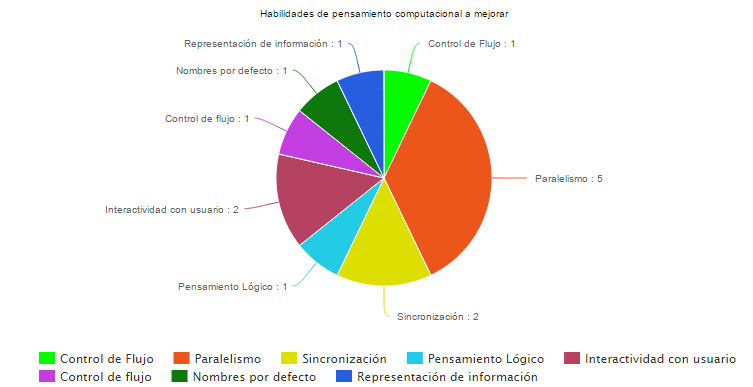
\includegraphics[bb=0 0 800 600, width=18cm, height=11cm, keepaspectratio]{habilidadestest.png}
	\caption{Habilidades de pensamiento computacional elegidas para mejorar}
  \label{figura:foro_hilos}
\end{figure}


%%%%%%%%%%%%%%%%%%%%%%%%%%%%%%%%%%%%%%%%%%%%%%%%%%%%%%%%%%%%%%%%%%%%%%%%%%%%%%%%
%%%%%%%%%%%%%%%%%%%%%%%%%%%%%%%%%%%%%%%%%%%%%%%%%%%%%%%%%%%%%%%%%%%%%%%%%%%%%%%%
% BIBLIOGRAFIA %
%%%%%%%%%%%%%%%%%%%%%%%%%%%%%%%%%%%%%%%%%%%%%%%%%%%%%%%%%%%%%%%%%%%%%%%%%%%%%%%%

\cleardoublepage

% Las siguientes dos instrucciones es todo lo que necesitas
% para incluir las citas en la memoria
%\bibliographystyle{unsrt}
%\bibliography{memoria}  % memoria.bib es el nombre del fichero que contiene
% las referencias bibliográficas. Abre ese fichero y mira el formato que tiene,
% que se conoce como BibTeX. Hay muchos sitios que exportan referencias en
% formato BibTeX. Prueba a buscar en http://scholar.google.com por referencias
% y verás que lo puedes hacer de manera sencilla.
% Más información: 
% http://texblog.org/2014/04/22/using-google-scholar-to-download-bibtex-citations/


 \begin{thebibliography}{1}

  \bibitem{note1} Django Project. {\em Página oficial del framework para el servidor} \\
	\url{www.djangoproject.com}

  \bibitem{note2} Bootstrap. {\em Página principal del framework de FrontEnd} \\
	\url{getbootstrap.com}

  \bibitem{note3} Hairball Framework. {\em Página oficial de Hairball}\\ 
	\url{gsyc.urjc.es} \\

	\bibitem{note4} Mozilla Add-on SDK. {\em Página oficial del SDK para desarrollo de 
	plugins Firefox} \\
	\url{developer.mozilla.org/es/docs/Mozilla/Add-ons/SDK}

  \bibitem{note5} Hairball. {\em Lint-inspired Static Analysis of Scratch Projects}: UC Santa Barbara. Boe Bryce, Hill Charlotee, Len Michelle.

 \end{thebibliography}


\end{document}
